%%%%%%%%%%%%%%%%%%%%%%%%%%%%%%%%%%%%%%%%%
% Masters/Doctoral Thesis 
% LaTeX Template
% Version 1.43 (17/5/14)
%
% This template has been downloaded from:
% http://www.LaTeXTemplates.com
%
% Original authors:
% Steven Gunn 
% http://users.ecs.soton.ac.uk/srg/softwaretools/document/templates/
% and
% Sunil Patel
% http://www.sunilpatel.co.uk/thesis-template/
%
% License:
% CC BY-NC-SA 3.0 (http://creativecommons.org/licenses/by-nc-sa/3.0/)
%
% Note:
% Make sure to edit document variables in the Thesis.cls file
%
%%%%%%%%%%%%%%%%%%%%%%%%%%%%%%%%%%%%%%%%%

%----------------------------------------------------------------------------------------
%	PACKAGES AND OTHER DOCUMENT CONFIGURATIONS
%----------------------------------------------------------------------------------------

\documentclass[11pt, oneside]{Thesis} % The default font size and one-sided printing (no margin offsets)

\graphicspath{{Pictures/}} % Specifies the directory where pictures are stored

\usepackage{comment}
\usepackage[square, numbers, comma, sort&compress]{natbib} % Use the natbib reference package - read up on this to edit the reference style; if you want text (e.g. Smith et al., 2012) for the in-text references (instead of numbers), remove 'numbers' 
\hypersetup{urlcolor=blue, colorlinks=true} % Colors hyperlinks in blue - change to black if annoying
\title{\ttitle} % Defines the thesis title - don't touch this

\begin{document}

\frontmatter % Use roman page numbering style (i, ii, iii, iv...) for the pre-content pages

\setstretch{1.3} % Line spacing of 1.3

% Define the page headers using the FancyHdr package and set up for one-sided printing
\fancyhead{} % Clears all page headers and footers
\rhead{\thepage} % Sets the right side header to show the page number
\lhead{} % Clears the left side page header

\pagestyle{fancy} % Finally, use the "fancy" page style to implement the FancyHdr headers

\newcommand{\HRule}{\rule{\linewidth}{0.5mm}} % New command to make the lines in the title page

% PDF meta-data
\hypersetup{pdftitle={\ttitle}}
\hypersetup{pdfsubject=\subjectname}
\hypersetup{pdfauthor=\authornames}
\hypersetup{pdfkeywords=\keywordnames}

%----------------------------------------------------------------------------------------
%	TITLE PAGE
%----------------------------------------------------------------------------------------

\begin{titlepage}
\begin{center}
\textsc{\LARGE \univname}\\[1.5cm] % University name
\textsc{\Large Master Thesis}\\[0.5cm] % Thesis type

\HRule \\[0.4cm] % Horizontal line
{\huge \bfseries \ttitle}\\[0.4cm] % Thesis title
\HRule \\[1.5cm] % Horizontal line
 
\begin{minipage}{0.4\textwidth}
\begin{flushleft} \large
\emph{Author:}\\
\href{http://www.johnsmith.com}{\authornames} % Author name - remove the \href bracket to remove the link
\end{flushleft}
\end{minipage}
\begin{minipage}{0.4\textwidth}
\begin{flushright} \large
\emph{Supervisor:} \\
\href{http://www.cmu.edu/iwess/people/volker-hartkopf.html}{\supname} % Supervisor name - remove the \href bracket to remove the link  
\end{flushright}
\end{minipage}\\[3cm]
 
\large \textit{A thesis submitted in fulfilment of the requirements\\ for the degree of \degreename}\\[0.3cm] % University requirement text
\textit{in the}\\[0.4cm]
\groupname\\\deptname\\[2cm] % Research group name and department name
 
{\large \today}\\[4cm] % Date
%\includegraphics{Logo} % University/department logo - uncomment to place it
 
\vfill
\end{center}

\end{titlepage}

%----------------------------------------------------------------------------------------
%	DECLARATION PAGE
%	Your institution may give you a different text to place here
%----------------------------------------------------------------------------------------

\Declaration{

\addtocontents{toc}{\vspace{1em}} % Add a gap in the Contents, for aesthetics

I, \authornames, declare that this thesis titled, '\ttitle' and the work presented in it are my own. I confirm that:

\begin{itemize} 
\item[\tiny{$\blacksquare$}] This work was done wholly or mainly while in candidature for a research degree at this University.
\item[\tiny{$\blacksquare$}] Where any part of this thesis has previously been submitted for a degree or any other qualification at this University or any other institution, this has been clearly stated.
\item[\tiny{$\blacksquare$}] Where I have consulted the published work of others, this is always clearly attributed.
\item[\tiny{$\blacksquare$}] Where I have quoted from the work of others, the source is always given. With the exception of such quotations, this thesis is entirely my own work.
\item[\tiny{$\blacksquare$}] I have acknowledged all main sources of help.
\item[\tiny{$\blacksquare$}] Where the thesis is based on work done by myself jointly with others, I have made clear exactly what was done by others and what I have contributed myself.\\
\end{itemize}
 
Signed:\\
\rule[1em]{25em}{0.5pt} % This prints a line for the signature
 
Date:\\
\rule[1em]{25em}{0.5pt} % This prints a line to write the date
}

\clearpage % Start a new page

%----------------------------------------------------------------------------------------
%	QUOTATION PAGE
%----------------------------------------------------------------------------------------

\pagestyle{empty} % No headers or footers for the following pages

\null\vfill % Add some space to move the quote down the page a bit

\textit{``My passion and great enjoyment for architecture, and the reason the older I get the more I enjoy it, is because I believe we - architects - can effect the quality of life of the people."}

\begin{flushright}
Richard Rogers
\end{flushright}

\vfill\vfill\vfill\vfill\vfill\vfill\null % Add some space at the bottom to position the quote just right

\clearpage % Start a new page

%----------------------------------------------------------------------------------------
%	ABSTRACT PAGE
%----------------------------------------------------------------------------------------

\addtotoc{Abstract} % Add the "Abstract" page entry to the Contents

\abstract{\addtocontents{toc}{\vspace{1em}} % Add a gap in the Contents, for aesthetics

  The project of Senior Community Center started from Fall 2014. The
  goal of the project is to 1) analyze the feasibility and the
  potential benefit of a Senior Community Center near CMU Campus, 2)
  conduct case review of related design with specific focus on
  inter-generational relationship creation.}

\clearpage % Start a new page

%----------------------------------------------------------------------------------------
%	ACKNOWLEDGEMENTS
%----------------------------------------------------------------------------------------

\setstretch{1.3} % Reset the line-spacing to 1.3 for body text (if it has changed)

\acknowledgements{\addtocontents{toc}{\vspace{1em}} % Add a gap in the Contents, for aesthetics

\par I would like to thank my advisor Prof. Volker Hartkopf for the guidance and help in establishing many connections.
\par I would like to thank Ms. Anne-Marie Lubenau for the kindly
sharing of her previous design of a Senior Community Center in the
proposed site.
\par I would like to thank Dr. Sharon Carver and Miss Allison Drash
from the children's school of Carnegie Mellon University who provided
valuable insights on the project.
\par I would like to thank Ms. Lyn Decker from Osher Lifelong Learning
Institute for her kindly help in helpping me understand more about the
life of the elderly and the potential opportunities and challenges.
\par I would like to thank Prof. Kristen Kurland for her comments and
ideas about the project and a list of valuable connections.
\par I would also like to thank Prof. Sean Qian for his guidance of me
through the GIS tools and the analysis method.  }
\clearpage % Start a new page

%----------------------------------------------------------------------------------------
%	LIST OF CONTENTS/FIGURES/TABLES PAGES
%----------------------------------------------------------------------------------------

\pagestyle{fancy} % The page style headers have been "empty" all this time, now use the "fancy" headers as defined before to bring them back

\lhead{\emph{Contents}} % Set the left side page header to "Contents"
\tableofcontents % Write out the Table of Contents

\lhead{\emph{List of Figures}} % Set the left side page header to "List of Figures"
\listoffigures % Write out the List of Figures

\lhead{\emph{List of Tables}} % Set the left side page header to "List of Tables"
\listoftables % Write out the List of Tables

%----------------------------------------------------------------------------------------
%	ABBREVIATIONS
%----------------------------------------------------------------------------------------

\clearpage % Start a new page

\setstretch{1.5} % Set the line spacing to 1.5, this makes the following tables easier to read

\lhead{\emph{Abbreviations}} % Set the left side page header to "Abbreviations"
\listofsymbols{ll} % Include a list of Abbreviations (a table of two columns)
{
\textbf{CMU} & \textbf{C}arnegie \textbf{M}ellon \textbf{U}niversity \\
\textbf{OSHER} & \textbf{A}cademy of \textbf{L}ifelong \textbf{L}niversity \\
\textbf{SCU} & \textbf{S}pecial \textbf{C}are \textbf{U}nit\\
%\textbf{Acronym} & \textbf{W}hat (it) \textbf{S}tands \textbf{F}or \\
}

%----------------------------------------------------------------------------------------
%	PHYSICAL CONSTANTS/OTHER DEFINITIONS
%----------------------------------------------------------------------------------------
\begin{comment}
\clearpage % Start a new page

\lhead{\emph{Physical Constants}} % Set the left side page header to "Physical Constants"

\listofconstants{lrcl} % Include a list of Physical Constants (a four column table)
{
Speed of Light & $c$ & $=$ & $2.997\ 924\ 58\times10^{8}\ \mbox{ms}^{-\mbox{s}}$ (exact)\\
% Constant Name & Symbol & = & Constant Value (with units) \\
}

%----------------------------------------------------------------------------------------
%	SYMBOLS
%----------------------------------------------------------------------------------------

\clearpage % Start a new page

\lhead{\emph{Symbols}} % Set the left side page header to "Symbols"

\listofnomenclature{lll} % Include a list of Symbols (a three column table)
{
$a$ & distance & m \\
$P$ & power & W (Js$^{-1}$) \\
% Symbol & Name & Unit \\

& & \\ % Gap to separate the Roman symbols from the Greek

$\omega$ & angular frequency & rads$^{-1}$ \\
% Symbol & Name & Unit \\
}
\end{comment}
%----------------------------------------------------------------------------------------
%	DEDICATION
%----------------------------------------------------------------------------------------

\setstretch{1.3} % Return the line spacing back to 1.3

\pagestyle{empty} % Page style needs to be empty for this page

\dedicatory{Dedicated to my family, friends and my instructors\ldots} % Dedication text

\addtocontents{toc}{\vspace{2em}} % Add a gap in the Contents, for aesthetics

%----------------------------------------------------------------------------------------
%	THESIS CONTENT - CHAPTERS
%----------------------------------------------------------------------------------------

\mainmatter % Begin numeric (1,2,3...) page numbering

\pagestyle{fancy} % Return the page headers back to the "fancy" style

% Include the chapters of the thesis as separate files from the Chapters folder
% Uncomment the lines as you write the chapters

% Chapter 1

\chapter{Background Information} % Main chapter title

\label{Chapter1} % For referencing the chapter elsewhere, use \ref{Chapter1}

\lhead{Chapter 1. \emph{Background Information}} % This is for the header on each page - perhaps a shortened title

%----------------------------------------------------------------------------------------

\section{Elderly Issue}
The commonly adopted boundary age for the elderly is 65 years old in
most of the developed counties~\cite{WHO2015}. From the 2010
U.S. census Demographic Profile Data, 13.1\% of the population are
over the age of 65. In Pittsburgh, this ratio is a little higher than
the nationwide statistics (\fref{fig:stat}, which is 13.8\% (42,151),
and 2.4\% (7347) of the population are of age over
85~\cite{censusQuickFact}. By 2030, 72.1 million (19\%) of the U.S
population will be elderly ~\cite{AOA2015}~
\begin{figure}[htbp]
  \centering
  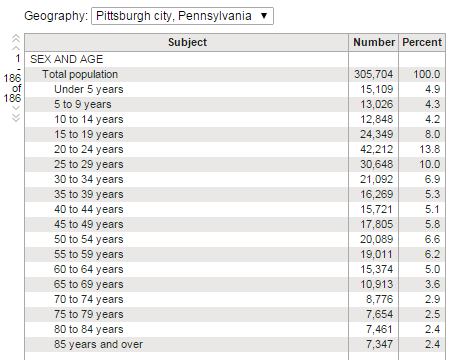
\includegraphics{stat.png}
  \caption[Demographic Information, Pittsburgh]{U.S. census 2010
    Demographic Profile Data (Pittsburgh)~\cite{censusQuickFact}}
  \label{fig:stat}
\end{figure}
%----------------------------------------------------------------------------------------

\par The awareness of the necessity for a senior community center near
Carnegie Mellon University Campus emerged from a previous course
project for Ecological Footprint in Fall 2013 conducted under
instruction of Prof. Hartkopf. In the analysis of the campus
neighborhood, the conflict between the relatively high ratio of senior
population around campus and a lack of proper facilities for senior
citizens was observed .

For imporving quality of life of the neighborhood as a whole,
providing access to safer, more affordable and more environmentally
friendly housing choices for students and faculty members and reducing
the travelling distance of faculty members to provide both more
sustainable and more affordable housing choices, a GIS analysis was
onducted

The series of analysis was conducted with ArcGIS
10.1~\cite{ArcGIS}. First the population density of senior citizen in
the surrounding neighborhood was calculated. The percentage of
population with an age above 65 was adopted as the metric of measuring
the concentration of senior population\cite{WHO2015}. From the
visualization of the senior population distribution, one can observe
that to the south of the campus, there is a large area with a very
high senior population percentage (Figure \ref{fig:seniorPopu}).
\begin{figure}[htbp]
  \centering
  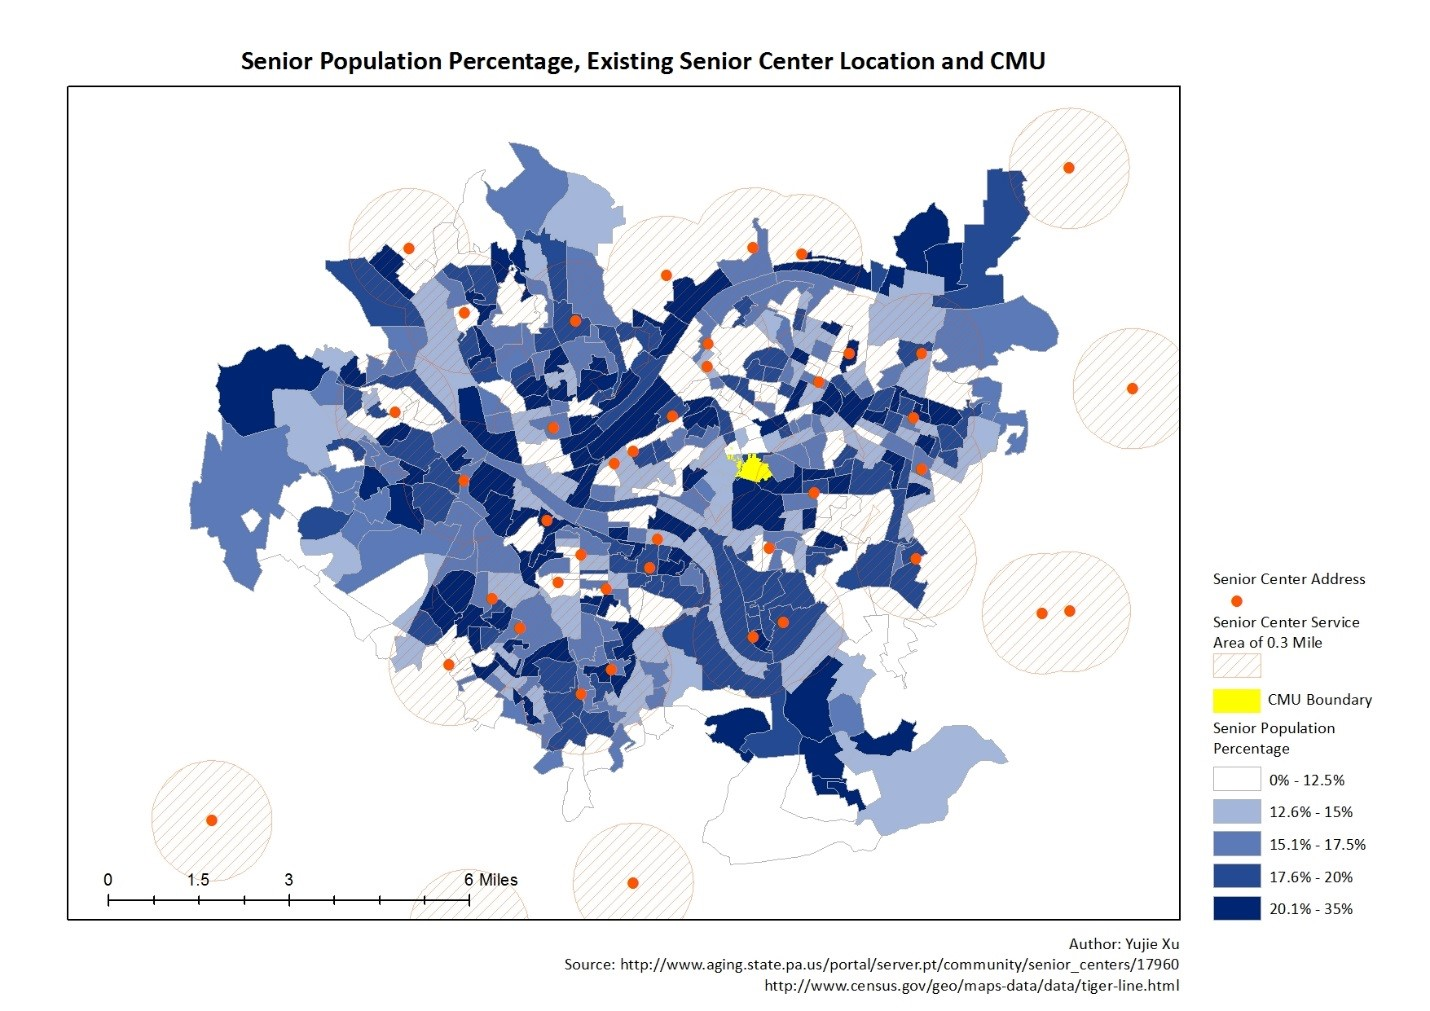
\includegraphics[scale=0.8]{seniorPopu.jpg}
  \rule{35em}{0.5pt}
  \caption[Near-campus Senior Population Density]{Senior Population
    Percentage, Existing Senior Center Location and CMU Campus
    Boundary}
  \label{fig:seniorPopu}
\end{figure}
Then the existing senior centers around Pittsburgh was located on the
map (\tref{tab:seniorCenter}~\cite{aging2013}). See Appendix A for a
list of senior centers located on the map~aref{AppendixA}. A 0.3 mile
service area buffer was created around each existing senior center
facility by applying the approximation analyze. A service area gab
around the campus where no senior center is within a proper walking
distance was identified.

This analysis acts as one of the reasons of the proposal of a senior
community center near CMU campus.

\section{Proposed Site}
\subsection{Surrounding Buildings}
The proposed site of the senior center is to the north of the CMU
campus next to Doherty Apartment across Forbes Ave. It is currently
a parking lot (\fref{fig:siteLocation}). To the north of the proposed
site is the East Campus Parking Garage. To the west of the site lie
the alumni house and the Fraternity/Sorority Quadrangle (\fref{fig:surroundingBd}).
\begin{figure}[htbp]
  \centering
  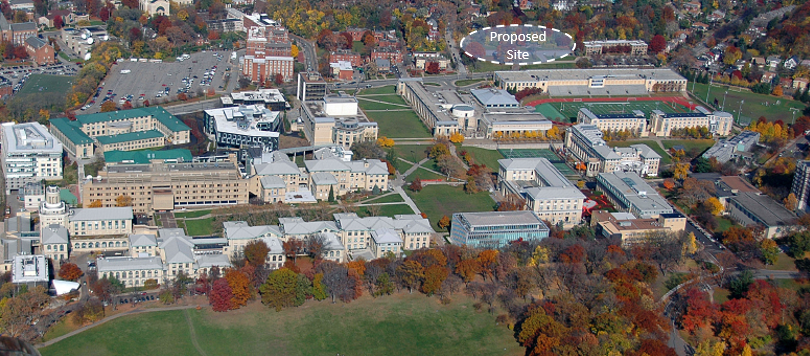
\includegraphics[width=0.7\textwidth]{siteLocation.png}
  \caption[Site Location]{Site Location Ariel View~\cite{masterplan}}
  \label{fig:siteLocation}
\end{figure}
\begin{figure}[htbp]
  \centering
  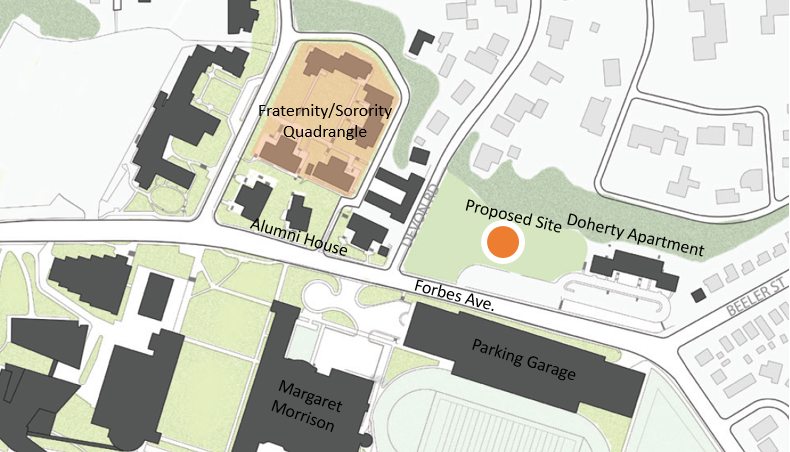
\includegraphics[width=0.7\textwidth]{surroundingBd.png}
  \caption[Surrounding Buildings]{Surrounding
    Buildings~\cite{masterplan}}
  \label{fig:surroundingBd}
\end{figure}
\subsection{Neighborhood Context}
The proposed site of the Senior Community Center is to the north of
Carnegie Mellon University, and is within the boundary of the
Squirrelhill North Neighborhood (\fref{fig:neighborhood}), which
contains the majority portion of the CMU campus. The remaining portion
of the campus is within the North Oakland neighborhood. 

The Squirrehlhill North Neighborhood is in an urban setting. Its
population density is 9713 person per square mile, much higher than
Pittsburgh average (5532). This indicates a less sprawled urban space
pattern and implies a higher chance of creating contact between the
elderly and the society. The neighborhood has a median household
income of \$82,214, over twice of that of the Pittsburgh
(\$35,947). The average household size is 2.1, These features suggest
the community of the proposed site is relatively wealthier and with
small household size. There are 16\% of foreign born residents. This
high ratio of foreign born residents suggest 1) the more urgent need
of a public life than a traditional community with mainly native
residents. The foreign born residents potentially has less social
contact than native residents and thus the community and social life
might be a more important aspect than native residents. 2) The design
of a new Senior Community Center should consider the cultural
difference of senior residents and should provide diversed services
that suits needs of different cultural background.  The area has a
much higher percentage of higher education attainment as a result of
the presence of Carnegie Mellon University.~\cite{neighborhood}
(\tref{tab:neighborStat})
\begin{table}
\begin{tabular}{ p{2in}|c c c c}
\toprule
&Squirrel Hill North&North Oakland&Pittsburgh\\
\midrule
Population Density (people per sq. mile)&9713&14658&5532\\
Median Household Income / \$&82214&40931&35947\\
Median Rent / \$&1123&603&760\\
Percentage of Family Household&45.4&10.9&37.7\\
Percentage of foreign born residents&16&27.5&7.4\\
Housing Price&516844&167225&132337\\
\bottomrule
\end{tabular}
\caption{Neighborhood Statistics}
\label{tab:neighborStat}
\end{table}

Average number of cars or other vehicles in the houses of neighborhood
is 2.2~\cite{neighborhood}. This ratio is high comparing with the
relatively small household size. It implies a less sustainable
traveling pattern. The design impact of the new senior center is that
it should both consider enough parking space, and also the ways to
demonstrate a sustainable travelling method by providing bicycle racks
and car-sharing facilities like a zipcar spot. The zipcar locations
near campus include the East Campus Garage and the parking lot to the
west of Morewood Gardens. 

The neighborhood is older than Pittsburgh average in terms of building
built year. The average estimated housing value (2010) for detached
houses are \$516,844, which is four times that of the Pittsburgh
average of \$132,337. The median rent is \$1,123, which is also a lot
higher than \$603 of Pittsburgh in genera. This rent price is
comparable to that of the renter occupied median housing cost in
Stanford, which indicates the necessity to provide housing for the
newly recruited faculty members (\tref{tab:midHousingcost}). 
\begin{figure}[htbp]
  \centering
  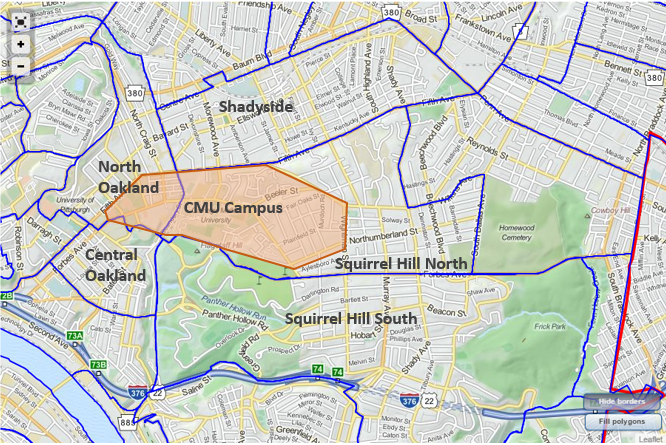
\includegraphics[width=0.7\textwidth]{neighborhood.png}
  \caption[Neighborhood]{Neighborhood Context of Proposed
    Site~\cite{neighborhood}}
  \label{fig:neighborhood}
\end{figure}

\begin{table}
  \begin{tabular}{c | c c c}
    \toprule
    Monthly Housing Cost (Median)	&Occupied	&Owner Occupied	&Renter Occupied\\
    \midrule
    Pittsburgh	&787	&820	&767\\
    Stanford	&1539	&2,933	&1,393\\
    \bottomrule
  \end{tabular}
  \caption{Median Monthly Housing Cost}
  \label{tab:midHousingcost}
\end{table}
\begin{comment}
\end{comment}
\subsection{Historic Aspect}
The site is vacant in 1900, from the history map in 1904, we can see a
brick structured building was present and the building belongs to M.C
Shiller. In 1959, Doherty Apartments is built [8] and has been
functioning ever since. This indicates there are no major historic
context needed to be reflected in the project design nor is there
important historic landmark on the site to be protected
(\fref{fig:history}).
\begin{figure}[htbp]
  \centering
  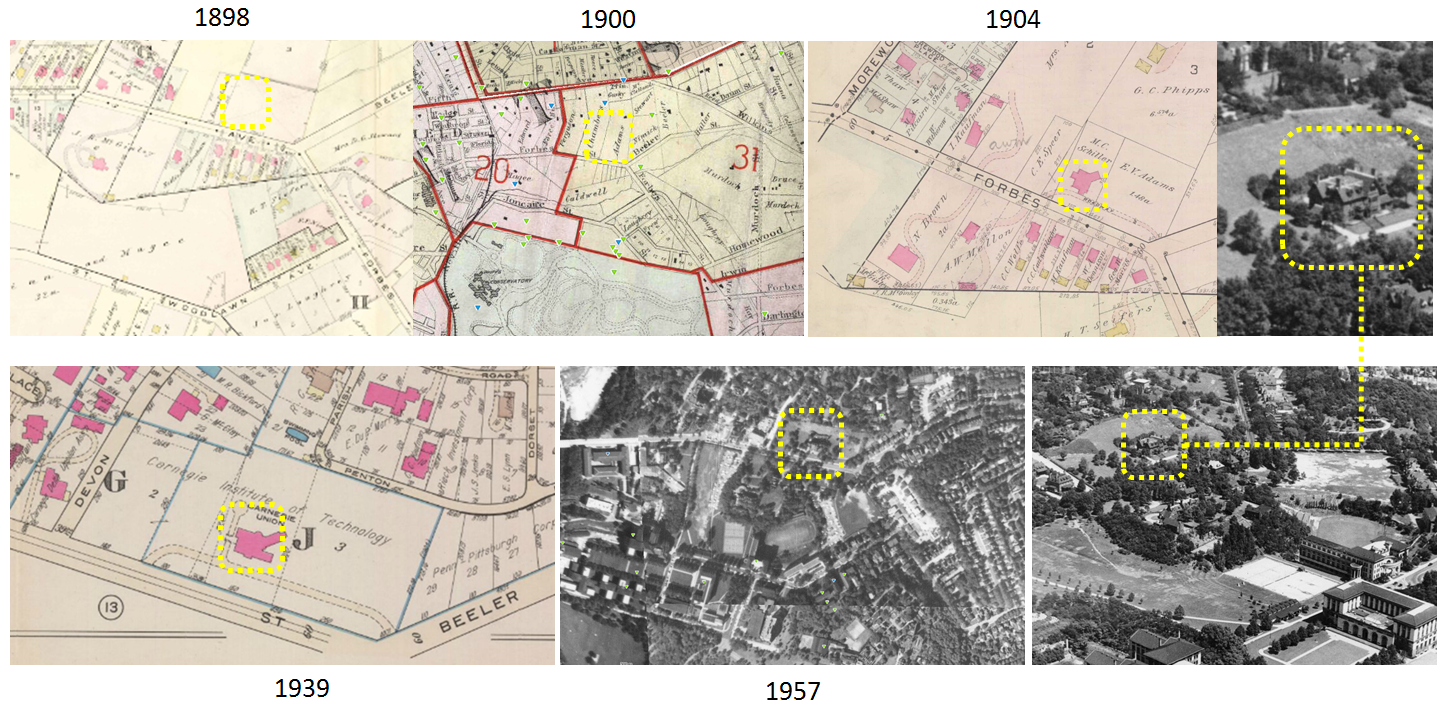
\includegraphics[width=\textwidth]{history.png}
  \caption[History of Site]{The History of the site from 1898 to 1957}
  \label{fig:history}
\end{figure}

\subsection{Physical Condition}
There is an elevation difference between the south and the north of
the proposed site. The north side is about 10m higher than that of the
south. The height difference created a stage for more varied landscape
design opportunities for creating connections between the senior
center, housing for elderly, and the Doherty appartment, housing for
young college students.

\section{Previous Design Conducted}
Ms. Anne-Marie Lubenau has completed a design of a senior center on
this site (~\fref{fig:prevDesign}). The general form of the building
consists of four major clusters: three major living cluster and one
public cluster. Each of the four cluster is easily identified with
the hipped roof above it. The public cluster locate on the
southwestern of the site and the remaining three living clusters
locate on the southeastern, northeaster and northwestern corner of the
building.

The public cluster consists of a public library, a group kitchen, a
lounge on the first floor, a computer cluster, a health suite on the
second floor and some mechanical rooms and storage rooms in the
basement. Each of the living cluster consists of 6 living unit per
floor except the first floor of the northeastern living cluster
consists only 4 living units. There are in total 54 living units in
the building. Between each of the adjacent cluster, there are some
lobby or lounge area. The vertical transportation located in the
center of each of the four cluster. There are 30 parking spot located
in the basement with the entrance on the northeastern corner of the
site.
\begin{figure}[htbp]
  \centering
  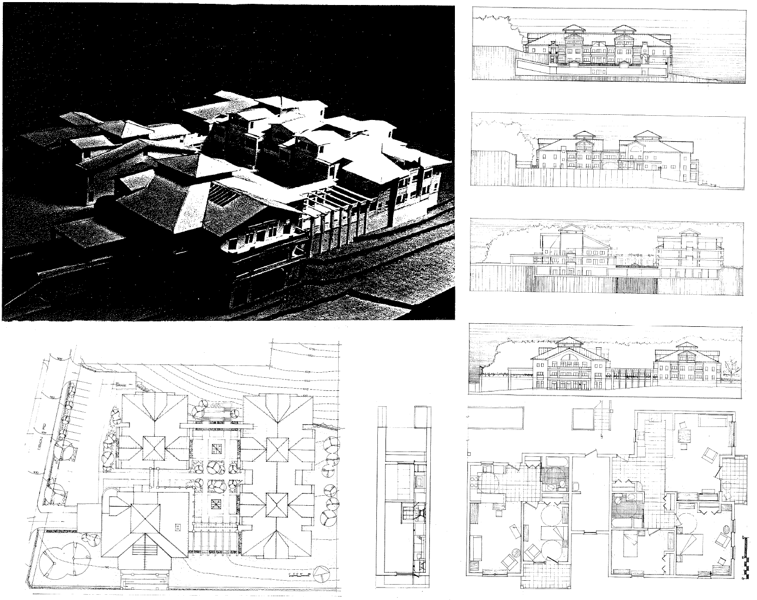
\includegraphics[width=\textwidth]{prevDesign.png}
  \caption[Design by Ms. Lubenau]{Senior Community Center Design by
    Ms. Anna Maria Lubenau}
  \label{fig:prevDesign}
\end{figure}
\section{Climate}
The site located in Pittsburgh, Pennsylvania. It is within the climate
zone 5A, with 5957 Heating Degree Day (HDD) of 65 $\deg F$ and 5009
Cooling Degree Day (CDD) of 74 $\deg$ F. The design heating
temperature is 8 $\deg F$ and design cooling temperature is 86
$\deg F$~\cite{remrate}

\section{Role of the Project}
\subsection{Bridge of Conversation between Different Age Group}
As is addressed by Neyfakh~\cite{Neyfakh2014}, American society is
confronted by severe age segregation, people are hashed into different
``buckets'' of ages groups and their social life is restricted to
their own ``bucket''. No more than 1/4 of the conversation about
``important matters'' happen between the elderly and people younger
than 36; by excluding relatives, the figure dropped to 6\%. Age
segregation ``sow distrust and prejudice between generations, and robs
people of the chance to learn from those younger and older than
them''~\cite{Neyfakh2014}.  The elderly benefit from reading to
children and children or the young people can learn the life knowledge
from the elderly.

One of the major focus of this project is to discuss methods to
establish an inter-generation connection. The role of architecture in
providing good quality of life for the elderly is far more than just
plugging in assisted living facilities and add some space for instant
medical care. It is also about creating chances of meeting new people
and about maintain the link to the society.

\subsubsection{Creating Connections between the Elderly and Children}
One of the elderly friend of Prof. Hartkopf shared his experience of
meeting children in their field trip. Children are the only people
that has the will to touch the elderly apart from the doctors that
give them a shot of drug when they get sick. The age group of elderly
is respected for their rich experiences along the development of
mankind, but is suffering from a segregation as a side-effect of the
development of the modern society.

The presence of a children’s school and the Academy of Lifelong
Learning (\href{http://www.cmu.edu/osher/}{OSHER}) on campus enables
the possibility to create a connection between the life of senior
citizens and the early education of the children in the children's
school.

\subsubsection{Creating Connections between Elderly and Student}
The proposed site is to the east of a student apartment, Doherty
Apartment. The design of a common space on roof level of the senior
center and the bridge from the senior center to the garage might
become a common route for both the elderly and the young colledge
students, which might be able to create interactions between the age
group of the elderly and young students.

Another approach to create the connections between these two age
groups is through volunteering programs where the students can
providing health or activity services for the elderly and the elderly
can also volunteer to participated in some of the study project of
students, especially in aging related areas.

In the discussion with directors in the childrens school, ``Lunchtime
Walking Buddy'' was brought up. It can be an example of how
volunteering opportunities can facilitate the connection between the
two age groups: The path between the proposed site of the senior
community center and the classroom of Lifelong Learning and the
Children's School will bypass the playground. Track walking is an easy
and effective physical exercise for both the elderly and the young. The
problem for the elderly is they might encounter sudden fall while
exercising. The volunteering lunchtime walking will benefit the
elderly by allowing a supervised safer exercise for the elderly and it
will benefit the young by providing them with the chance of
conversation with people of rich life experiences.

Yet another approach is through providing some well designed common
spaces. For example, the common space on the top level of the senior
center could provide a nice study space and the basement will contain
some extra music practicing rooms which might attract young student to
come and use, and thus creating chances for the young and old to meet.

\subsection{Center for Geriatrics (Aging Related) Researches}
There are several geriatrics research groups in or around Carnegie
Mellon University. The creation of such a center near campus can
provide more interactions and hands-on experience with their research
target and thus might assist the development of the related
researches.

\subsubsection{Connections to Quality of Life Technology (QoLT) Center}
The focus of the QoLT center is ``intelligent systems that improve
quality of life for everyone while enabling older adults and people
with disabilities''~\cite{QoLT2014}. One of the promising research
branch of the QoLT center that facilitates the connection to the
Seniro Center is one of the four Testbed Systems: the Home and
Community Health \& Wellness (HCHW), whose goal is described as ``The
goals of the Home and Community Health \& Wellness (HCHW) testbed
systems are to create and evaluate home and community-based solutions
for assessing everyday functional status, providing appropriate
feedback, and assisting rehabilitation in the natural environment for
people with reduced capabilities due to disability or aging.  HCHW
systems will enable more older adults and people with disabilities to
live independently. ''~\cite{HCHW}

The following are some project carried on by the HCHW system:
\begin{itemize}
\item Health Kiosk\\
  The Health Kiosk system allows the elderly to track and record their
  health conditions including ``blood pressure, blood oxygen level,
  handgrip, weight, hearing'' etc. and remotely send the results to
  clinicians without an actual clinical visit. It provides senior
  citizens with easy monitoring and knowledge of their health
  conditions on a regular basis (~\fref{fig:kiosk})~\cite{Kiosk}.
 \begin{figure}[htbp]
   \centering
   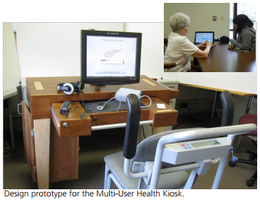
\includegraphics[width=0.5\textwidth]{kiosk.png}
   \caption[Health Kiosk]{Health Kiosk~\cite{Kiosk}}
   \label{fig:kiosk}
\end{figure}
\item Embedded Assessment of Wellness with Smart Home Sensors\\
  The system helps to monitor the abilities of senior citizens in
  performing everyday activities and provides information of the
  degree of physical ability
  declination.~\cite{Lee:2010:EAW:1864431.1864490}
\end{itemize}

\subsection{Community Center for the Elderly and Other Residents}
Although the proposed senior center will contain some amount of living
units to the elderlies with various degree of assistance: from the
active independent elderly, to those need intensive assistance to
those with special needs of assistance (Alzheimer Disease) even the
``end-of-life'' issue. One of the important roles of the center is to
act as a community gathering space dedicated for the surrounding
neighborhood.

\subsection{Demonstration of Advanced Building Technology and System
  Design}
\subsubsection{Urban Agriculture}
Gardening / Horticulture is one of the shared activities of almost all
age groups . It can create food, jobs and a chance of meeting and
mixing of different age groups. Possible approaches of the project on
Urban Agriculture include:
\begin{itemize}
\item Create Roof Gardens on the top floor of the parking garage and
  part of the Senior Community Center

The benifits of using green roof include: reducing stormwater runoff,
protecting roof membrane, reducing heating/cooling load and reducing
urban heat island effect~\cite{Snodgrass2010}.
\item Create Vegetation facade for the Senior Community Center
\end{itemize}
These green space will act as a stage for common activities of
children and elderly to happen; a place to hide from the noise of the
urban jungle; a field to produce food and a classroom for teaching
healthy eating habbits.

\subsubsection{Sustainable / Renewable Energy Source}
\begin{itemize}
\item Solar Energy for electricity: 
  \begin{itemize}
  \item Integration of PV panels and green roofs.
  \item Integration of PV panels and shading devices
  \end{itemize}
\item Geothermal
\item Co-generation system within the building groups
\end{itemize}
\subsubsection{Passive Strategy}
\begin{itemize}
\item Design of building orientation and dimension of space to
  facilitate day-lighting and natural ventilation

Ensure all living units have a south facing window.
\item Rainwater collection and reuse
\item Phase-changing material
\end{itemize}
\subsubsection{Pre-fabrication of Building Components}
\begin{itemize}
\item Using steel or alluminum as the main building structure material.
\item Use a common mode for building design to minimize the number of
  distinct elements.
\end{itemize}
%\subsubsection{Intelligent Building Control System}
\subsubsection{Strategies for Maximizing the Indoor Environment Quality}
\begin{itemize}
\item Water-based heating and cooling system to ensure both the energ performance and the acoustic quality of the indoor environment 
\item Floor-based mechanical system to ensure low pollutant concentration and space flexibility  
\item Transparent space boundary design to allow views to indoor and outdoor activities and to create spatial guidance for the elderly.
\item Installing Personal Environment Module to account for stricter environment requirement from the elderly.
\end{itemize}
\begin{comment}
\section{Benefit for the Elderly}
\subsection{Fighting Age Segregation}
It creates opportunities for fighting "age segregation", a severe problem in the U.S. life style, and facilitates the integration of different age groups.
\subsection{High Quality Continued Education}
\subsection{Adjacency to Art and Culture}
\subsection{Mobility and Green Lifestyle}
\end{comment}
\section{Design Choices and Concerns for Children and Elderly}
Through the discussion with the administrators of the
\href{http://www.psy.cmu.edu/cs/}{children's school} of Carnegie
Mellon University,
Ms. \href{http://www.psy.cmu.edu/cs/people/carver.html}{Sharon
  Carver}, Director of Children's School, and
Ms. \href{http://www.psy.cmu.edu/cs/people/drash.html}{Allison Drash},
the Administrative Coordinator, a lot of insights were acquired about
different approaches about how children and elderly can be related.
\subsection{Integrated Learning Opportunities}
\subsubsection{Dalcroze Eurhythmics}
Music is a common activity shared by all age groups including the elderly and the young children. It is not only a delight for life but also a effective training for brain and physical dexterity development for children and the function maintenance of the elderly. One of such example is the Dalcroze Eurhythmics. It teaches music concepts through body movements.

Eurhythmics is a good candidate for creating common activities between the elderly and the children because: 1) it involves plenty of body movement which can be game-like for children and can be good exercise for the elderly 2) Marta Sanchez Dalcroze Training Center in Carnegie Mellon University has a high quality education in Dalcroze Eurhythmics that offers classes for both the children and the elderly.
\subsubsection{Elderly Reading to Children}
A nursing home in Tulsa, Grace Living Center has a collaboration with the Jenks public school. The facility provids two classrooms for 60 kindergarton students  of grade 1 and 2 and preschool students. The elderly residents in the center can volunteer to become mentors for the children that assists children in both acadamic and social development. Children brought joy in elderly's life, and the elderly provided acadamic improvement for children. The Jenks school found that ``a smaller percentage of students from the GLC have required reading intervention'' in their later studies. One example of the collaborated learning is the ``book buddies'' activities, where children and elderly form groups and read to each other severa times per week. Another example is the ``shared study'', where the elderly and the children work on craft activities together such as making Christmas ornaments, scarecrows etc. There are also comparative course content when the elderly and children share their lifes of ``then and now'' \cite{Morehouse2009}.
\begin{figure}[htbp]
  \centering
  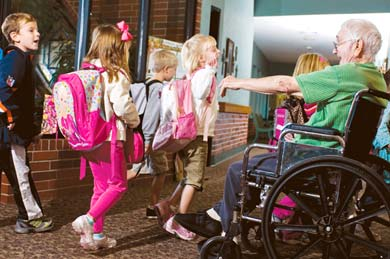
\includegraphics[width=0.5\textwidth]{oldAndYoung.jpg}
  \caption[Ageless Friendship]{Elderly meet School Children at Grace
    Living Center, Tulsa~\cite{Parker2009}}
  \label{fig:oldAndYoung}
\end{figure}
\subsubsection{Horticulture}
The term ``gray and green'', introduced by Wright and
Lund, means the positive effect of introducing
green plants on the process of aging. Gardening reduces stress,
nurtures stewardship~\cite{Wright2000229}. Gardening activities is one
of the common activities that benifit both the children and the
elderly. The ``edible garden'' is mentioned by Tai et al.\ in the book
Designing Outdoor Environments for Children. Edible gardens can let
children experience the whole gardening process from growing to
harvest, promote physical activities and also teach children the
knowledge of healthy eating, which contributes to the battle towards
childhood obesity in the U.S~\cite{Tai2006}, which shortens children's
lifespan expectancy by five years~\cite{Souterbrown2015}. They also mentioned a
type of ``music garden'', where outdoor music instrument are
incorporated in the design of garden environment.

Green space can also act as a healing and conforting power. There are
two major types of such salutogenicly designed gardens: the ``healing
or sensory garden'' that provide passive assist to imporve healthy
conditions. ~\cite{Souterbrown2015}. The ``Healing Gardens'' aims at
providing a quiet and calming space away from urban environment noise,
where ``young and old can escape and emotionally revitalise''. The
``Sensory Garden'' provide a ways to open up the senses of visitors{:
visually, acoustically, variety in scents, tastes and touching
experiences. ``Therapeutic Gardens'' actively conduct healing
operations. There are specific therapeutic gardens for people with
dememtia or mobility problem. A common feature of such therapeutic
gardens is raised bed, which is accessible for people in a wheel
chair.

\subsection{Mobility Issue}
The mobility is a big issue that needs to be seriously dealt with for
the two age groups to meet and have common activities. The elevation
difference, staircases and busy roads can all potentially become
barriers that prevents them from using the path we
designed. Especially for children, in order to reach the proposed site
of the senior center, they have to cross Forbes Ave. According to the
safety requirement, the children need to cross the street with the
presence of traffic lights, so the possible places to cross are either
the crossing at Forbes and Beeler or at Forbes and Morewood. Such
detouring can increase the travel distance and may cause the failure
of establishing such a connection, especially when there are not
enough cleaning and resting facilities as chairs and bathrooms along
the path.

The presence of university center along the path is a great
help. Since the building itself is already a well functioned and
energetic gathering space that provides abundant cleaning and resting
spaces.

One of the desired solution for the detouring and the crossing of
Forbes Ave. is to create a bridge that directly connects the
university center and the senior center. This solution can both
shorten the distance and fulfill the required services along the
path. But from the location of the University Center and the proposed
site, the bridge directly connecting both will be too long to
construct. So instead I propose to connect the parking garage with the
senior center. This bridge may not only act as a safe cross for the
senior people, children as well as the students living in Doherty
Apartment, but also an identification of the entrance to the campus
zone.

The parking garage needs to be retrofitted so that it will not become
an unpleasant spot along the route that only creates noise and exhaust
gas, but a great view. This will be further discussed in the section
of the proposed design of the plants and green space in the senior
center and along the path between senior center and children school.

% Chapter 3

\chapter{Case Study} % Main chapter title

\label{Chapter2} % For referencing the chapter elsewhere, use \ref{Chapter1} 

\lhead{Chapter 2. \emph{Case Studies}} % This is for the header on each page - perhaps a shortened title

%----------------------------------------------------------------------------------------

\section{General Design Considerations of Senior Population}
Senior center is an active node in the community that supply resources
to senior citizens and provide the community with aging related
knowledge~\cite{Dalsanto2009}. Main services offered at a senior
center include: education on a broad range of topics including health,
art, humanity, nutrition etc., volunteering opportunities,
intergeneration programs, meal plans, health screening, physical
training etc. 

There are several main categories of housing choices for the elderly:
independent living communities, assisted living facilities, Continuing
Care Retirement Communities (CCRC), nursing homes, and special care
facilities as Alzheimer's care facilities. The main difference are the
degree of care provided. Residents of independent living communities
differ from normal communities mainly in the demographic sence,
i.e. the residents are limited to senior citizens. Assisted living had
24 hour staff and provide living services such as meal, laundry and
bathing. It is meant for seniors that are not capable of living
independently but are not in need of heavy medical care. Nursing home
are more like hospitals with on site physicians and nurses that
provide high degree of medical care in addiction to living
services. CCRC provides varied degrees of service that covers all the
services provided in the housing types above and may include some
dementia care~\cite{JFCS2015}. Due to the awareness of the negative
impact of relocation of seniors especially those with dementia, the
CCRC prototype for senior living is the most suitable in the current
case.

The senior community center under discussion in the current project is
a combined community center and housing for senior citizens. It also
integrates with the university population by providing common space to
the community including university population, some housing units for
newly enrolled faculty members and space for elderly-children common
activities with the children from the children's school or from the
community. These makes the function different from a traditional
senior center setting. The case study in this section focus more on
the aspect specific to the project, such as the instances with mixed
age groups, affiliated to a university, or a combined facility of
living and research.

\section{Elderly and Children Combined Facility}
\subsection{Multi-generational Neighborhood Center}
In Europe, ``multi-generational neighborhood centers''
are alternatives to traditional senior centers that creates
inter-generational connections. The services expanded from traditional
senior center to include pre-school and infant care etc~\cite{Fromm2015}. 

\subsubsection{Intergenerational Quartier (Germany)}
The IGZ Quartier urban regeneration project is located in the city of
D{\"u}lmen. The Intergenerational Center of the project aims at ~\cite{Dulmen2014}
!!!!!!!!!!!!!!!!!
\subsection{Mixed-generation Elderly Housing}
In Swabia, Germany, a housing program for elderly was created with 2/3
elderly residents and 1/3 of other age groups. The housing model aims
at helping elderly age in place with helps from other generations in a
``supportive environment''. The common space is extensible and can
hold a variety of activities arranged by social workers and the
residents themselves. The activites take place in the common space
include: morning play of children, affordable lunch for both the
senior residents and people from the neighborhood, informal community
gatherings and rent out space for other community events~\cite{Fromm2015}.

\subsection{Elderly Housing Next to Kindergarten}
\subsubsection{Altersheim Furttal, A Retirement Home in a Swiss Village}
The retirement home is built near the city center with good public
transportation. This connection provides the residents with a stronger
connection to the society.

There is a kindergarten to the north of the facility. The connections
between the two age groups are established with a common courtyard
between the kindergarten and the retirement home. The interior space
design strengthens this connection by arranging a two story ``lounge
space'' adjacent to the common garden.

\begin{figure}
\centering
\begin{subfigure}{0.7\textwidth}
  \centering
  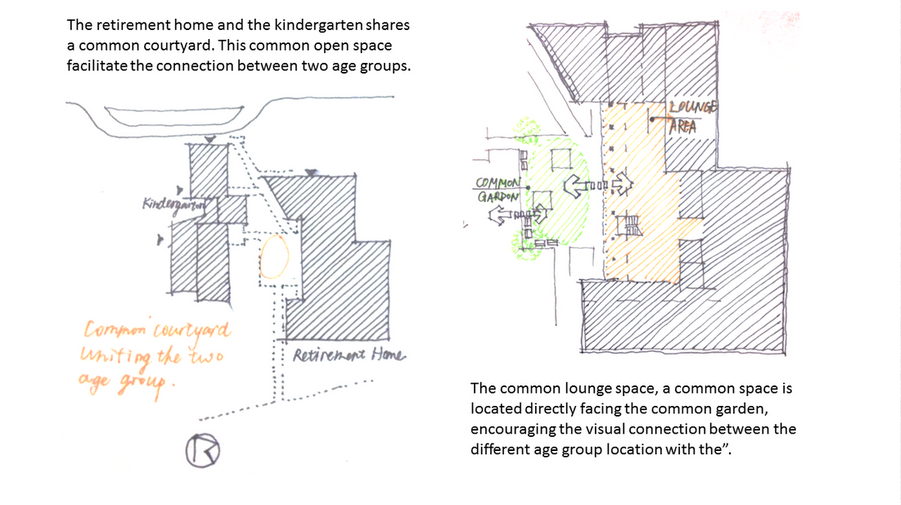
\includegraphics[width=\linewidth]{case1.png}
  \caption{Site Plan Layout of Altersheim Furttal and Kindergarten}
  \label{fig:case1}
\end{subfigure}
\begin{subfigure}{0.7\textwidth}
  \centering
  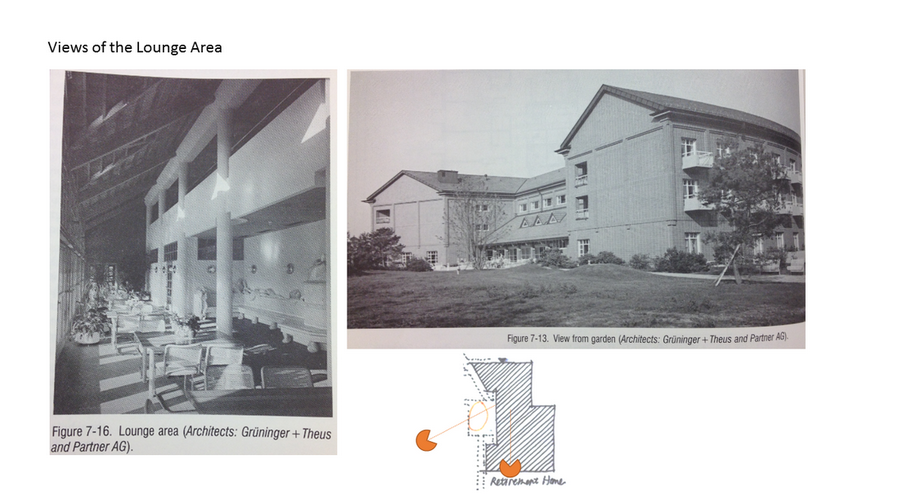
\includegraphics[width=\linewidth]{case2.png}
  \caption{Views of the Lounge Area}
  \label{fig:case2}
\end{subfigure}
\caption{Common Garden and Interior Design in Creating Connections
  between Different Age Groups}
\label{fig:case2}
\end{figure}
\section{University Affiliated Senior Housing}
\section{Dementia Assisted Living}
``Dementia is an umbrella term for a group of cognitive disorders
typically characterized by memory impairment, as well as marked
difficulty in the domains of language, motor activity, object
recognition, and disturbance of executive function – the ability to
plan, organize, and abstract.''~\cite{CDCdementia} Dementia, or its
most common form Alzheimer is highly prone and one could not neglect
its existance: there are 5 million Alzheimer victims in the U.S. and
every 1 out of 3 seniors die in dementia. Women are more vulnerable to
dementia and 2/3 of the Alzheimer victims are
women~\cite{alzorg2014}. This section conduct some related case study
on elderly caring facilities for people with Alzheimer Diseases. 

The physical space acted as a ``therapeutic resource'' in improving
the wellbeing and help reduce the seriousness of
dementia~\cite{Day2000}. Relocation of individual dementia victims to
new environments can increase the possibility of depression and
mortality~\cite{ANTHONY01111987}. This implies the necessity for
dementia dedicated space. If there are not such spaces, when resident
develops dementia, they will have to be relocated to facilities that
has dementia care functions, which might cast negative impact. The
living unit for cognitively impared people are commonly refered to as
Spetial Care Unit (SCU). The common features of SCUs include ``smaller
size units, fewer resident rooms and more designated private rooms
with private dining rooms''. The SCU environment have positive impact
on ``communication, self-care, social function and mobility'' status
of dementia victims. It also reduce emotional strain and increase
satisfactions. Separation between people with and without dementia is
necessary as study showed non-dementia residents experience mental
declines as a result of living near dementia victims. The tipical
features of a SCU unit include: less rooms, small room sizes, private
rooms and dining space, access to outdoor environment
etc~\cite{Day2000}. Smaller cluster size showed positive effects on
reducing agitation level, aggressiveness, anxiety and
depression~\cite{Day2000}. The positive impact of smaller cluster
group setting also includes relief of stress and negative attitude of
relative care-givers~\cite{Annerstedt19931529, Day2000}. Special
acoustic feature should be added to create a balance between ``sensory
overstimulation'' and ``deprivation'', i.e. create a space that is
neither too noisy nor too quiet. Since people with dimentia tend to
also have visual difficulties, the suggested visual environment is low
glare, high contrast and increase lighting level~\cite{Day2000}. The
``bright light treatment'' showed improvement on sleep
patterns~\cite{Mishima1994}. For enhancing way-finding, common design
suggestions include: provide views to the outside environment which
gives hint of location; create ``landmarks'', large signs; increase
lighting level of public spaces etc. Corridors are associated with
less orientation and higher percentage of hallway reduces
disorientation~\cite{Day2000}
\section{Sustainable Strategy in Senior Center} 
% Chapter3

\chapter{Preliminary Design} % Main chapter title

\label{Chapter3} % For referencing the chapter elsewhere, use \ref{Chapter1} 

\lhead{Chapter 3. \emph{Preliminary Design}} % This is for the header on each page - perhaps a shortened title

%----------------------------------------------------------------------------------------
\section{Design Specification}
\subsection{Major Functions}
There are four major functions of the senior community center project:
\begin{enumerate}
\item Providing housing units to elder population in the surrounding
  communities and newly enrolled faculty members. Providing choices of 
  various degrees of care and the special care of Aalzheimer's
  disease. 
\item As a result of the collaboration with the OSHER (Lifelone
  Learning Center), providing classrooms and administrative officies
  for OSHER. 
\item Providing labs for aging related researches.
\end{enumerate}
\subsection{Degree of Care for the Elderly}
There are eight major building types of senior care / housing program:
geriatric clinic, out patient clinic, adult day care, nursing home
(long term care), independent living, assisted living, and facilities
for people with Alzheimer's Disease. The first two options only
provides medical or consulting services for elderly that encounters
congnitive, physical or emotional problems, the adult day care mainly
serves people with cognitive problems and cannot stay at home by
themselves. It normally operates between 8 to 5. It acts as an
alternative to assisted living and long-term care~\cite{seniorLiving}.

\section{Site Planning}
The site plan of the building consider to create a bridge between the senior center and the parking garage. It provides an entrance on the top floor of the senior center facing east, so that the student from the Doherty Apartment can use the public space on the top floor and the bridge to cross the Forbes Ave~\fref{fig:bridge}.
\begin{figure}
\centering
\begin{subfigure}{0.7\textwidth}
  \centering
  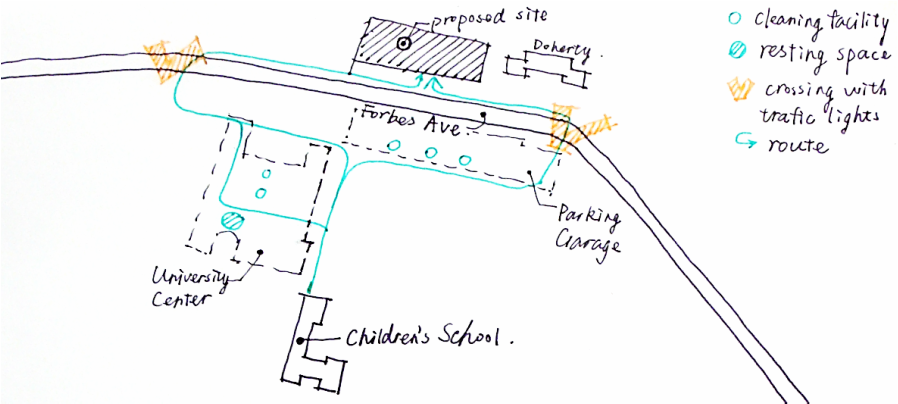
\includegraphics[width=\linewidth]{bridge1.png}
  \caption{Detouring Path from Children's School to the Proposed Site}
  \label{fig:bridge1}
\end{subfigure}
\begin{subfigure}{0.7\textwidth}
  \centering
  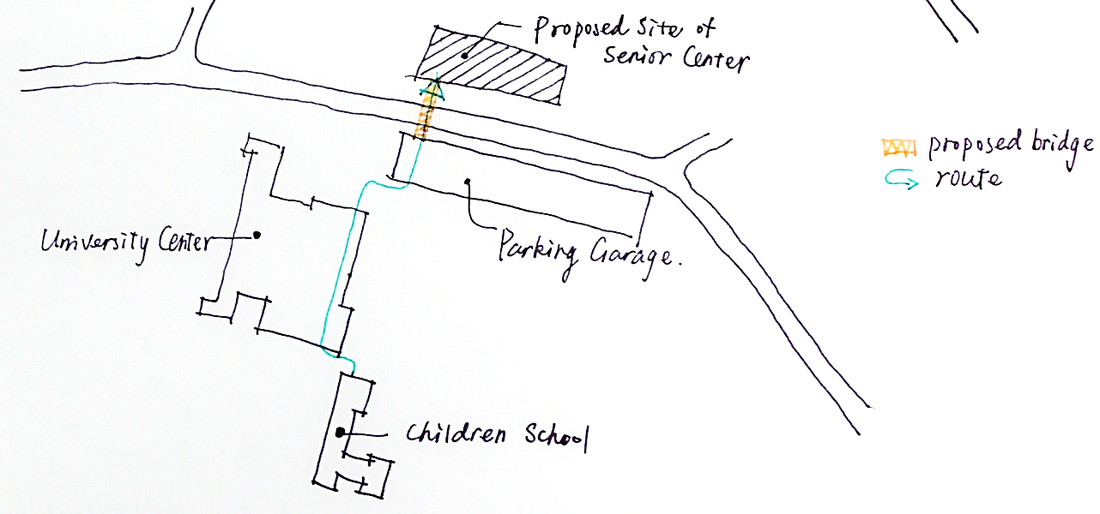
\includegraphics[width=\linewidth]{bridge2.png}
  \caption{Creating a Bridge to Reduce Detouring Distance}
  \label{fig:bridge2}
\end{subfigure}
\caption{Bridge Connecting Parking Garage and Senior Center}
\label{fig:bridge}
\end{figure}

\begin{figure}
\centering
\begin{subfigure}{\textwidth}
  \centering
  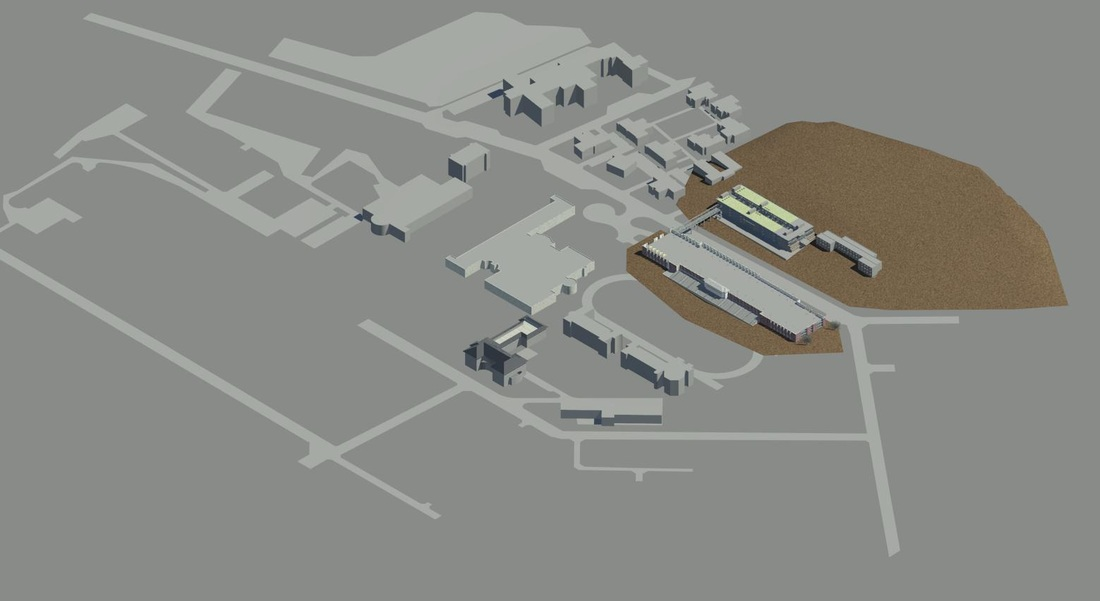
\includegraphics[width=0.9\textwidth]{site.jpg}
  \caption[Site Planning]{Site Planning Perspective View}
  \label{fig:site}
\end{subfigure}
\begin{subfigure}{\textwidth}
  \centering
  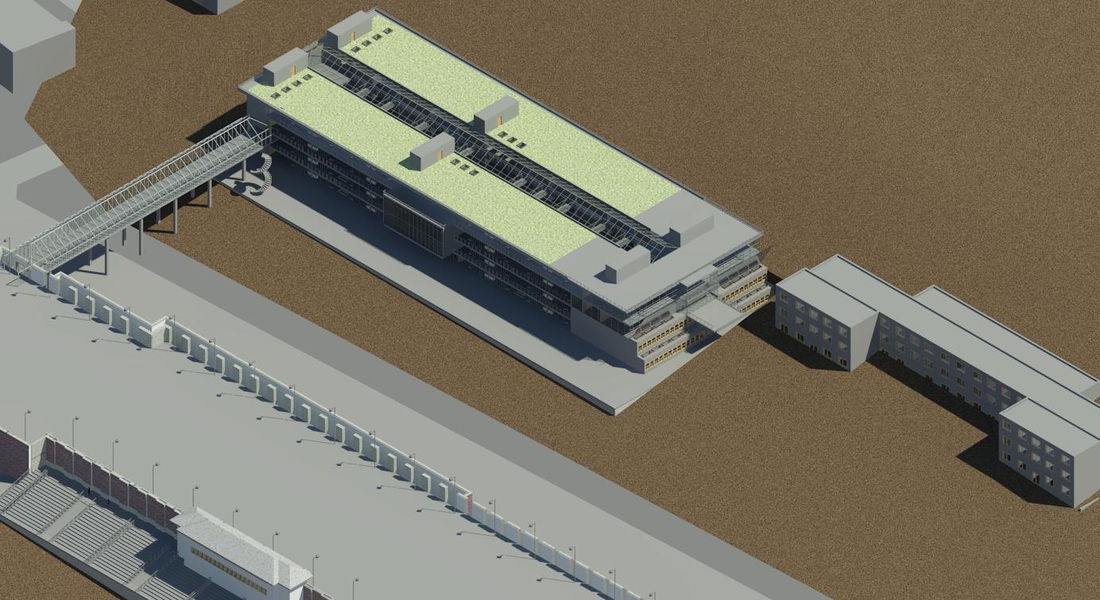
\includegraphics[width=0.9\textwidth]{siteClose.jpg}
  \caption[Site Planning Closer View]{Site Planning Closer View}
  \label{fig:siteClose}
\end{subfigure}
\caption{Site Planning}
\label{fig:siteAll}
\end{figure}
\section{Living Unit and Group Design}
\subsection{Topological Pattern of Living Cluster Design}
There are two aspects of aging: the ``biological process'' and the
``social passage''. For the social passage, as one become aged, one
tends to encounter a dramatic change in the social roles, some tends
to withdraw from previous responsibilities, some seeks to engagement
in new social roles~\cite{Perkins2004}. Providing a soft transition
and a variety of choices is a key to maintain a balance between the
social connection and the degree of privacy. Upon this concern, the
basic space structure of public-private-transition is defined
recursively as follows.

Another reason to organize space in this pattern is to encourage a
group-assist living pattern, to encourage residents to give and
receive help from their neighbors and the living group, which can both
provide a sense of self-achievement for helping others, to prolong
the time of transferring to a higher nursing degree and to strengthen
bounds between residents.

Another concern is especially for higher degree of living care, the
varied degree layout facilitates privacy in care-giving and
receiving with small nursing group.

Yet another consideration is to assign each group a common space and
encourage the residents to arrange the decoration and space
functionality, which increases the sense of belonging.
\begin{figure}
\centering
\begin{subfigure}{0.7\textwidth}
  \centering
  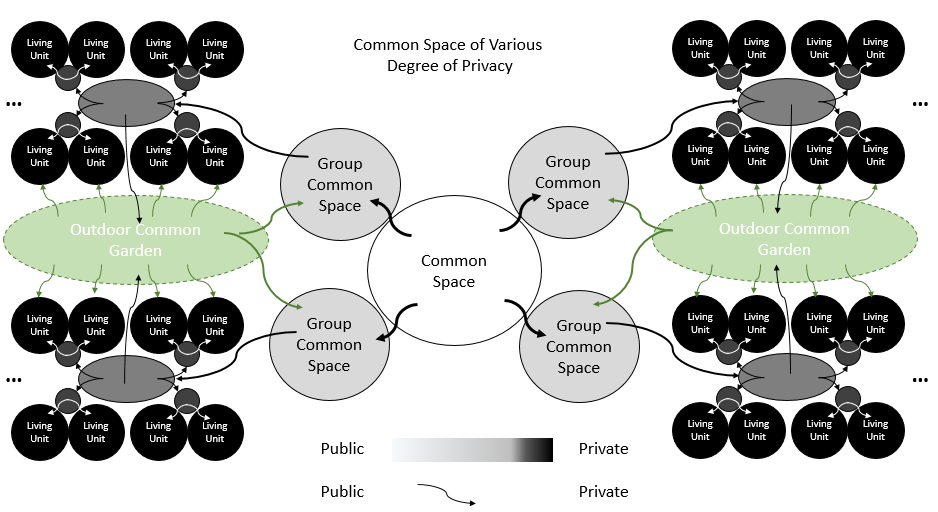
\includegraphics[width=\linewidth]{spacePattern.png}
  \caption{Space Pattern: Soft Transition of Public and Private Space}
  \label{fig:spacePattern}
\end{subfigure}
\begin{subfigure}{0.7\textwidth}
  \centering
  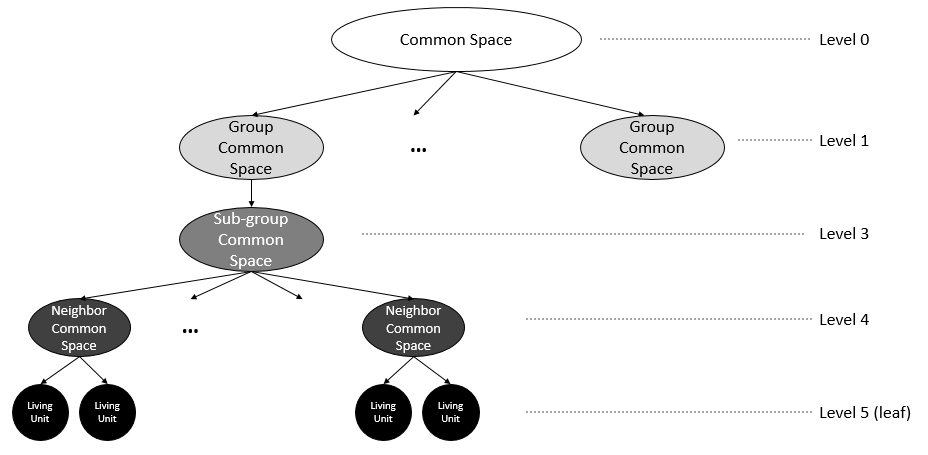
\includegraphics[width=\linewidth]{spaceTree.png}
  \caption{Tree Representation of Degree of Privacy Level}
  \label{fig:spaceTree}
\end{subfigure}
\caption{Space Pattern of Privacy Level Transition}
\label{fig:spacePrivacy}
\end{figure}
\subsection{Design Living Unit}~
\begin{figure}[htbp]
	\centering
		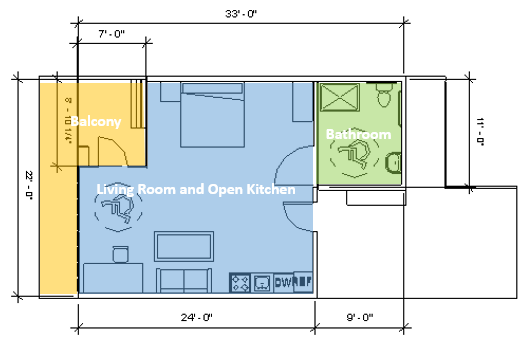
\includegraphics[width=0.7\textwidth]{plan1unit.png}
	\caption[Plan of Living Unit]{Plan of Living Unit}
	\label{fig:plan1unit}
\end{figure}
\begin{figure}[htbp]
	\centering
		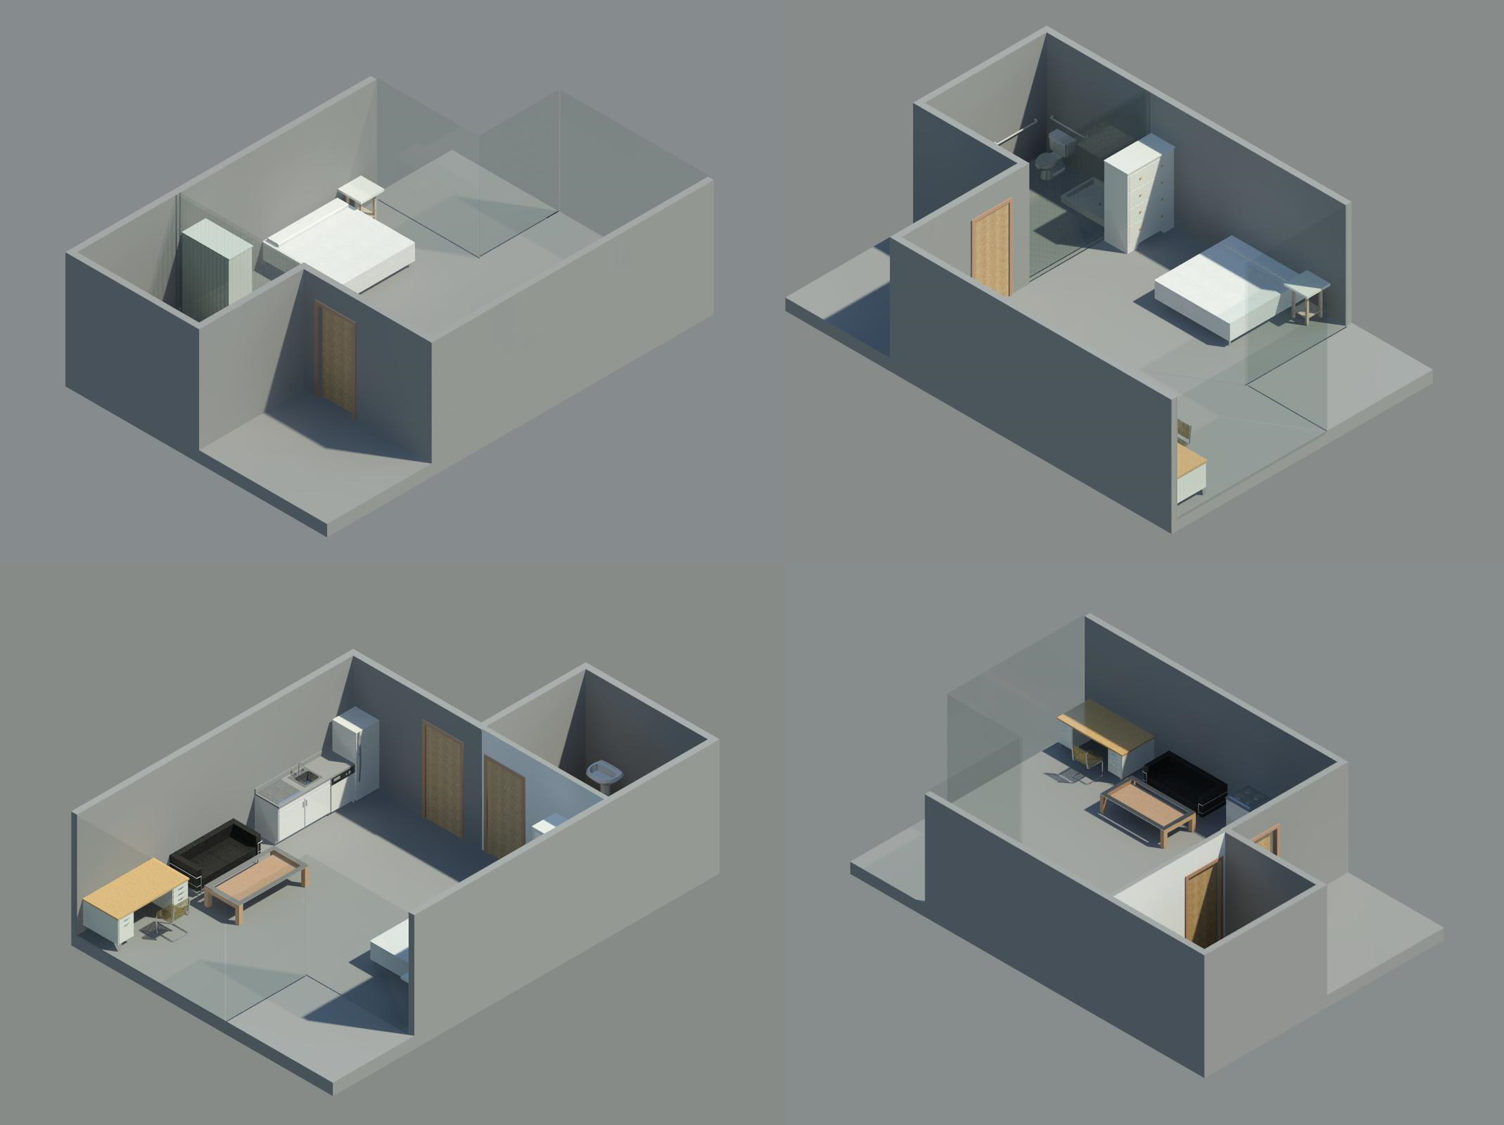
\includegraphics[width=\textwidth]{persUnit.png}
	\caption[Perspective View of Living Unit]{Perspective View of Living Unit}
	\label{fig:persUnit}
\end{figure}
\subsection{Living Unit Group and Common Space Design}
\begin{figure}[htbp]
	\centering
		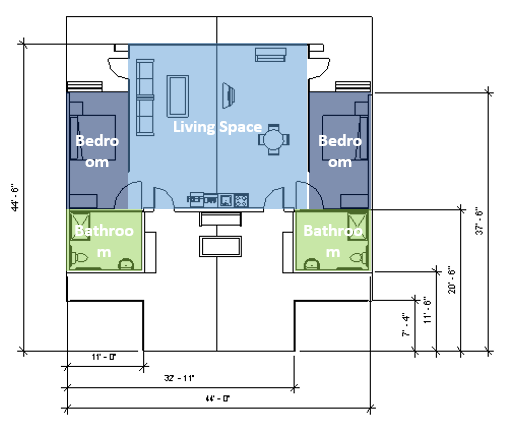
\includegraphics[width=0.7\textwidth]{plan2unit.png}
	\caption[Plan of Two-Unit Group]{Plan of Two-Unit Group}
	\label{fig:plan2unit}
\end{figure}
\begin{figure}[htbp]
	\centering
		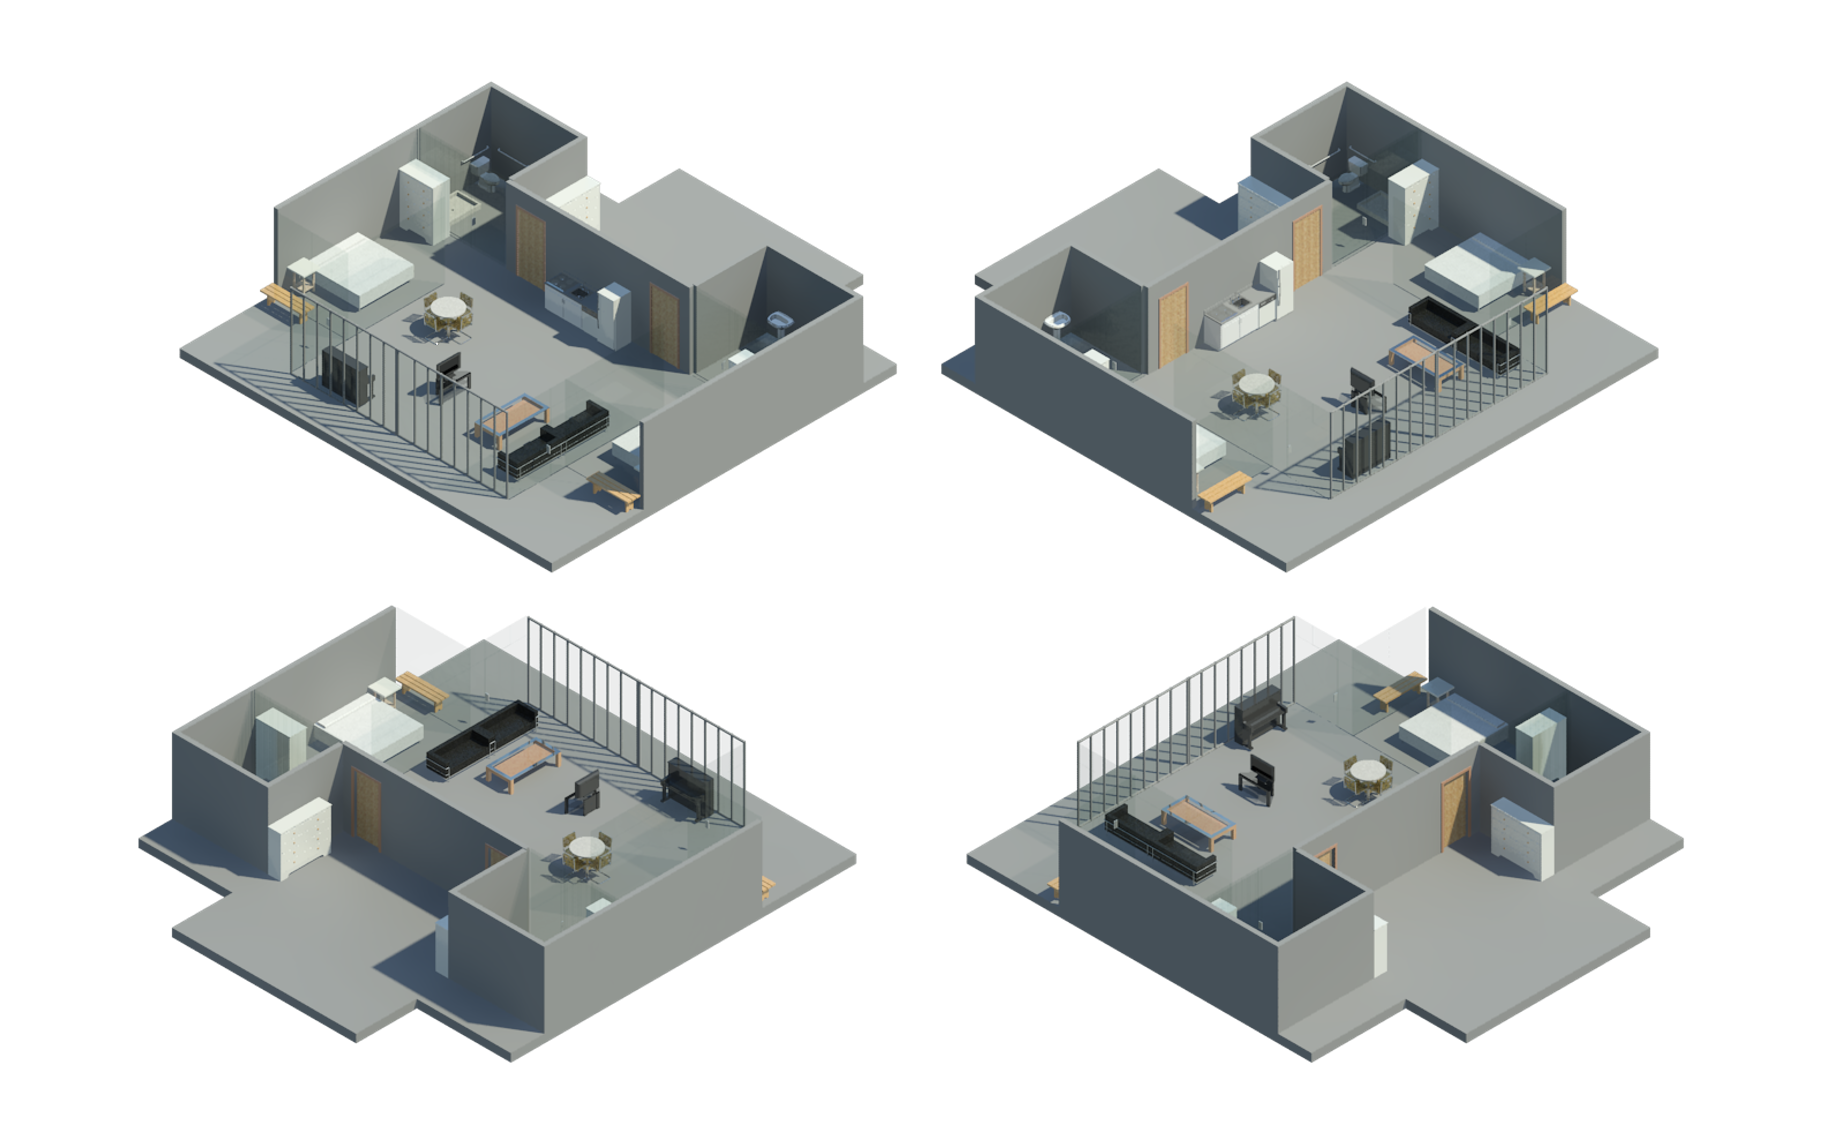
\includegraphics[width=\textwidth]{pers2unit.png}
	\caption[Perspective View of Two-Unit Group]{Perspective View of Two-Unit Group}
	\label{fig:pers2unit}
\end{figure}
\begin{figure}
\centering
\begin{subfigure}{\textwidth}
  \centering
  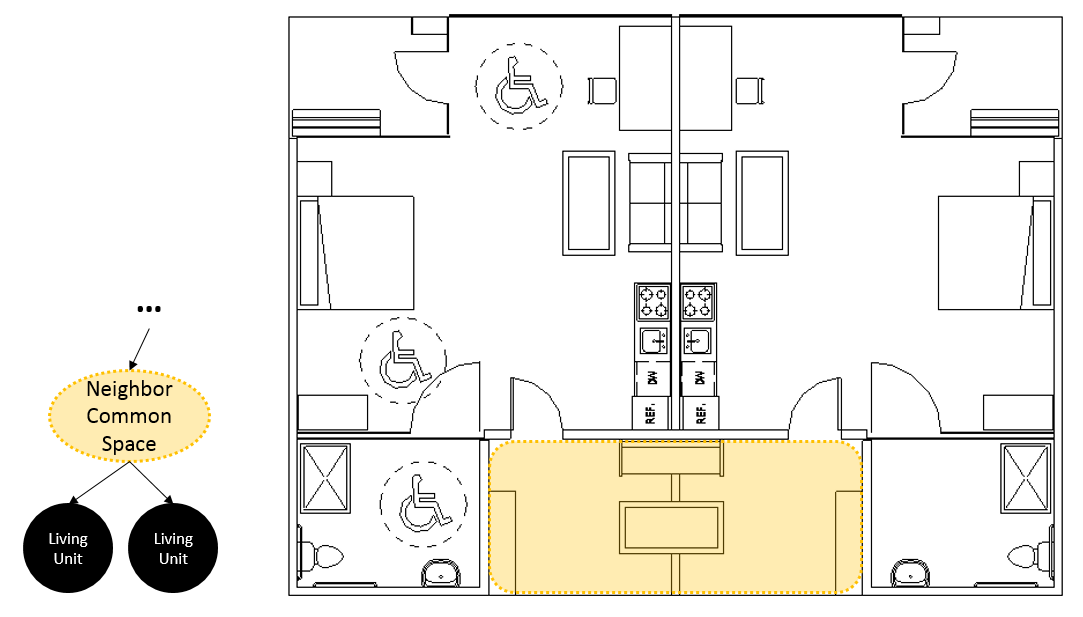
\includegraphics[width=\linewidth]{twoUnit-1.png}
  \caption{Common Space of Two Unit: Common Entrance}
  \label{fig:twoUnit-1}
\end{subfigure}
\begin{subfigure}{\textwidth}
  \centering
  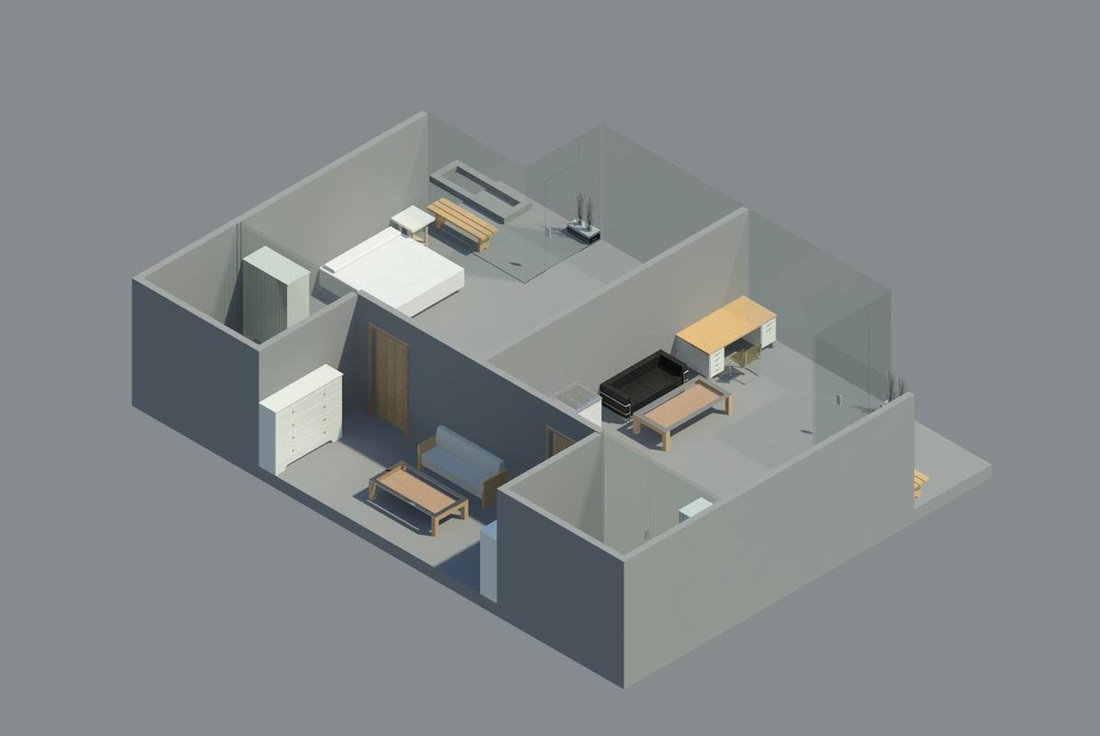
\includegraphics[width=\linewidth]{twoUnit-entrance.jpg}
  \caption{Perspective View of Common Space of Two Unit: Common Entrance}
  \label{fig:twoUnit-entrance}
\end{subfigure}
\caption{Two Unit Common Space}
\label{fig:twoUnitCommonSpaceEntrance}
\end{figure}

\begin{figure}
\centering
\begin{subfigure}{\textwidth}
  \centering
  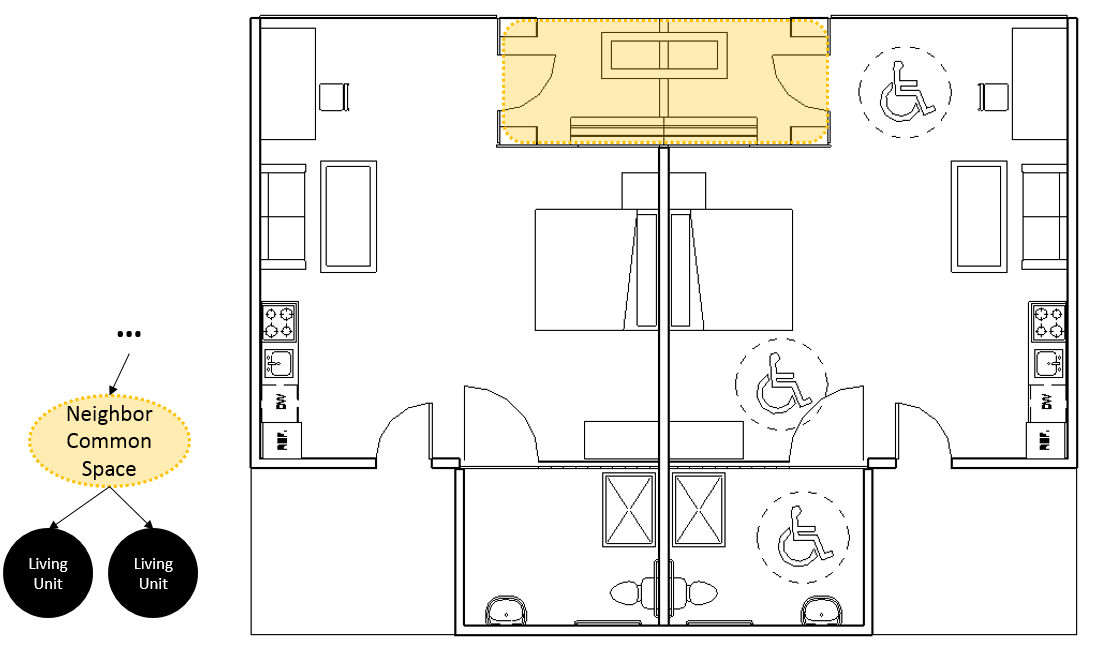
\includegraphics[width=\linewidth]{twoUnit-2.png}
  \caption{Common Space of Two Unit: Common Garden}
  \label{fig:twoUnit-2}
\end{subfigure}
\begin{subfigure}{\textwidth}
  \centering
  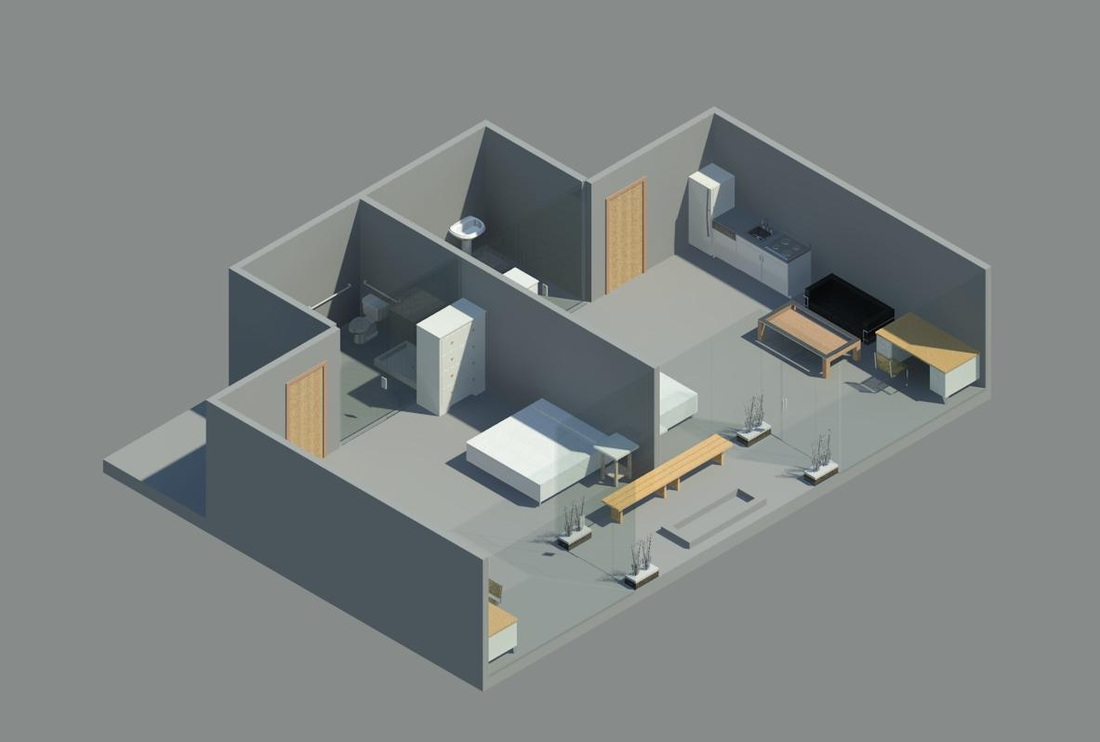
\includegraphics[width=\linewidth]{twoUnit-gd.jpg}
  \caption{Perspective View of Common Space of Two Unit: Common Garden}
  \label{fig:twoUnit-garden}
\end{subfigure}
\caption{Two Unit Common Space}
\label{fig:twoUnitCommonSpaceGarden}
\end{figure}

\begin{figure}
\centering
\begin{subfigure}{\textwidth}
  \centering
  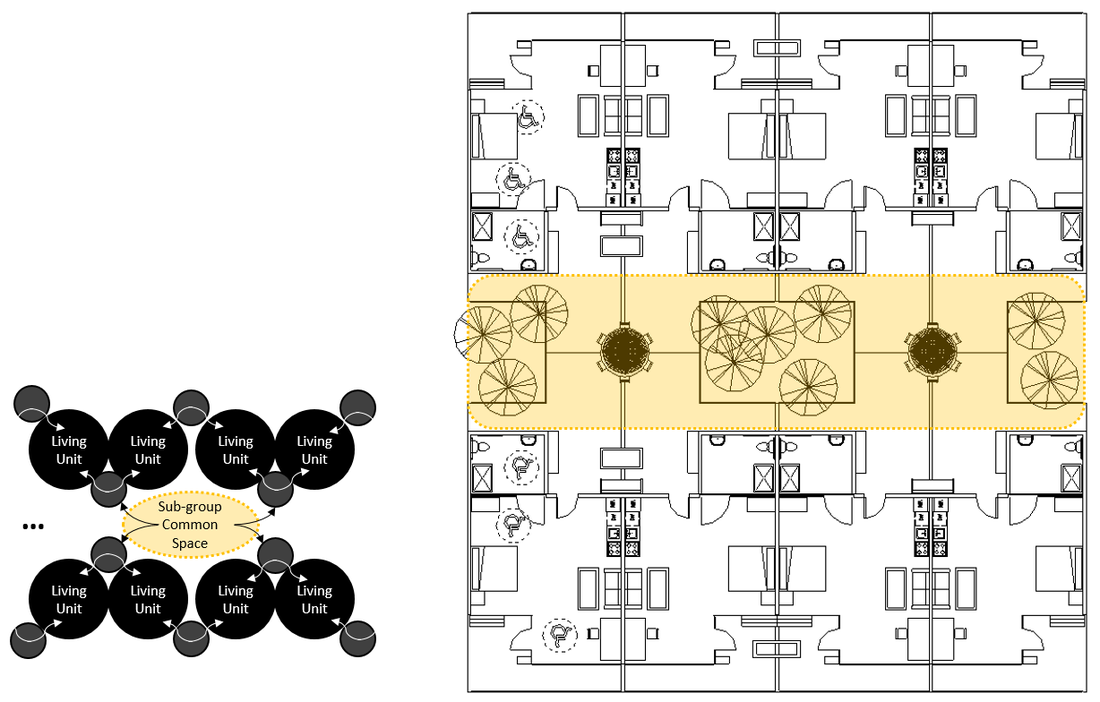
\includegraphics[width=\linewidth]{commonSpace8.png}
  \caption{Common Space of Eight Unit}
  \label{fig:commonSpace8}
\end{subfigure}
\begin{subfigure}{\textwidth}
  \centering
  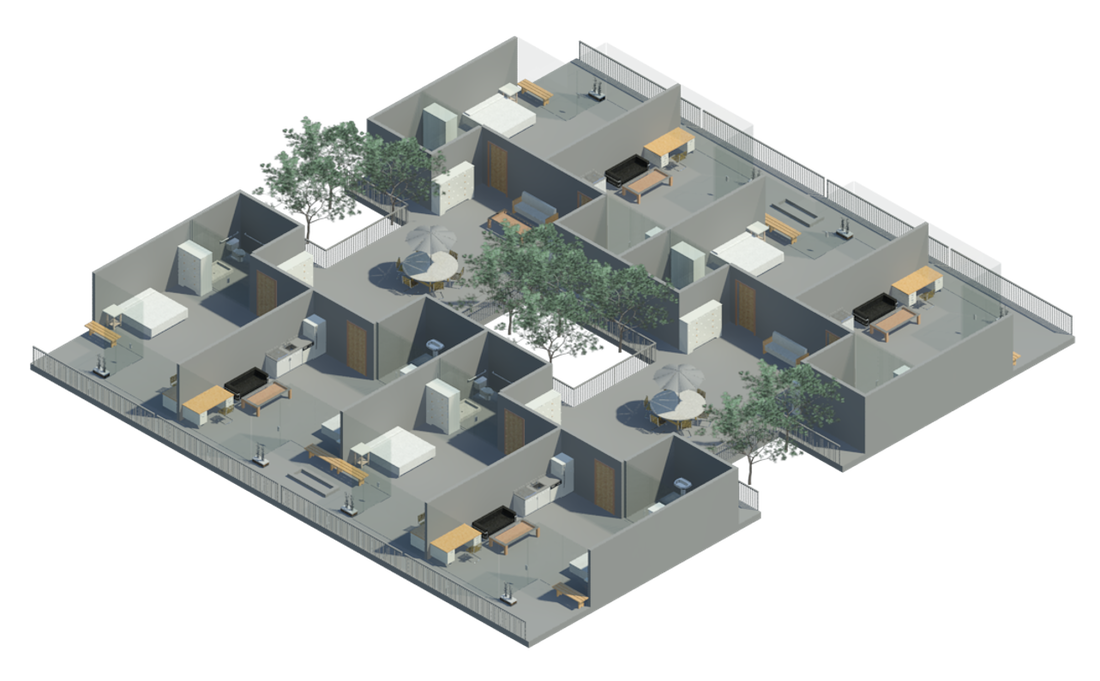
\includegraphics[width=\linewidth]{commonSpace8pers.png}
  \caption{Perspective View of Common Space of Eight Unit}
  \label{fig:commonSpace8pers}
\end{subfigure}
\caption{Eight Unit Common Space}
\label{fig:eightUnitCommonSpace}
\end{figure}

\begin{figure}
\centering
\begin{subfigure}{\textwidth}
  \centering
  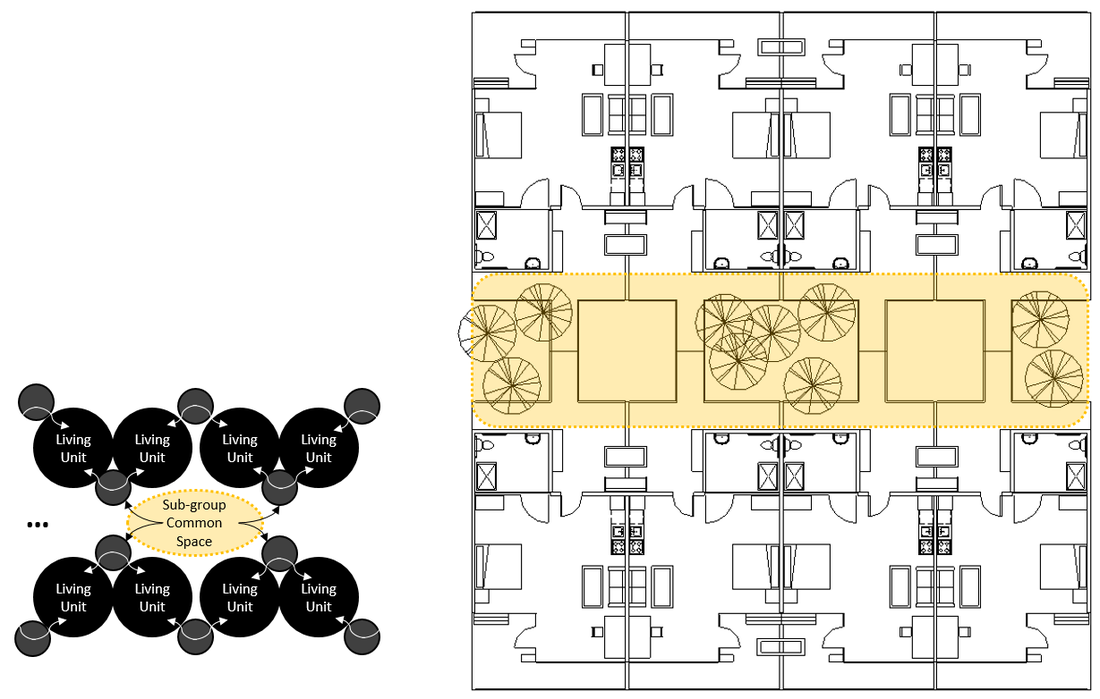
\includegraphics[width=\linewidth]{commonSpace8up.png}
  \caption{Common Space of Eight Unit: Upper Level}
  \label{fig:commonSpace8}
\end{subfigure}
\begin{subfigure}{\textwidth}
  \centering
  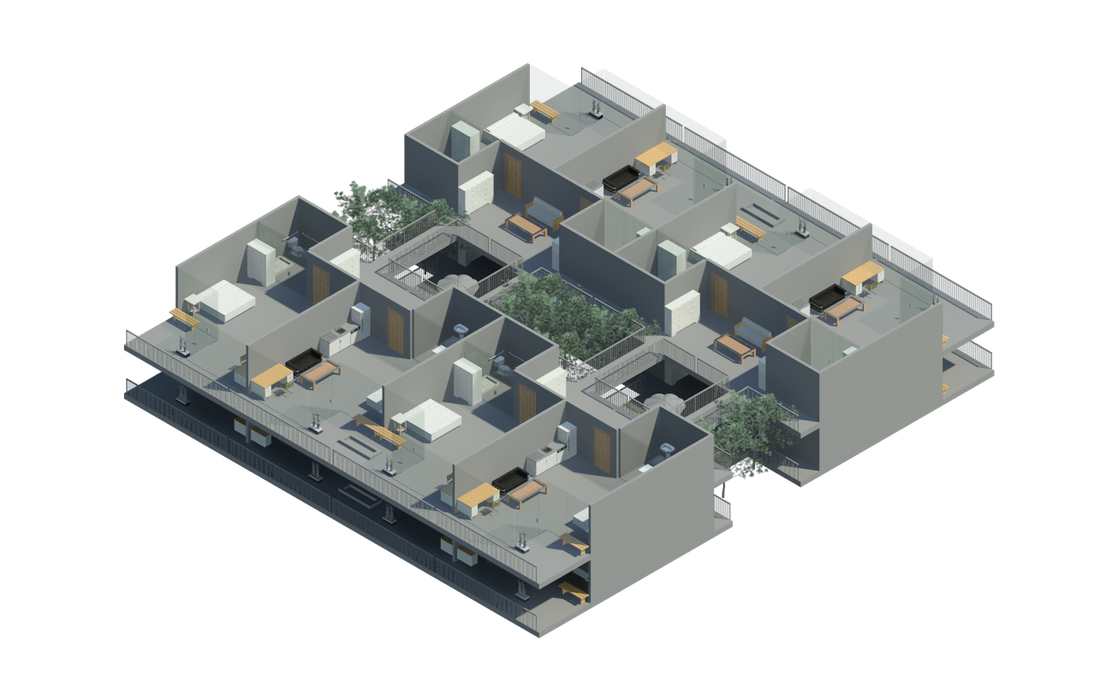
\includegraphics[width=\linewidth]{commonSpace8upPers.png}
  \caption{Perspective View of Common Space of Eight Unit: Upper Level}
  \label{fig:commonSpace8pers}
\end{subfigure}
\caption{Eight Unit Common Space: Upper Level}
\label{fig:eightUnitCommonSpaceUp}
\end{figure}

\newpage
\section{Path Arrangement}~
The major concern for path design includes:
\begin{itemize}
\item To create more chance of encountering people, both the elderly residents and the young people.
\item To accommodate the needs for the Alzheimer Disease victims. \\A ``wandering loop'' (\fref{fig:path}) is needed to accomodate the behavior change for the Alzheimer Disease victims. For more detailed information, please refer to the case study in \cref{Chapter3}
\end{itemize}

\begin{figure}[htbp]
	\centering
		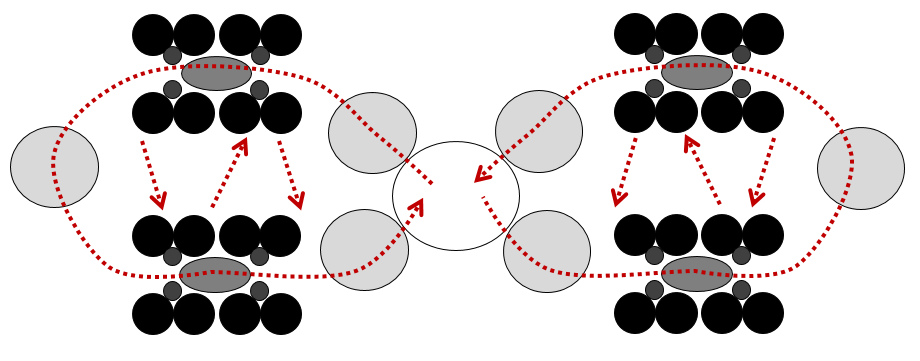
\includegraphics[width=0.7\textwidth]{path.png}
	\caption[Path Pattern]{Path Pattern}
	\label{fig:path}
\end{figure}
\subsection{Access to Nature}
In order to allow for easy access to nature, the indoor garden is created between each of the two major row of living units, allowing for access to nature in the indoor environment~\fref{fig:indoorGarden}.
\begin{figure}[htbp]
	\centering
		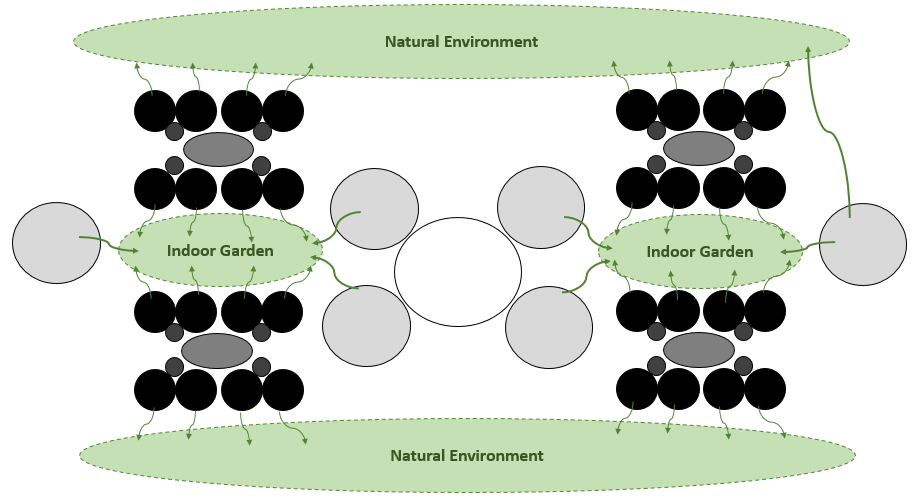
\includegraphics[width=0.7\textwidth]{indoorGarden.png}
	\caption[Access to Nature]{Access to Nature}
	\label{fig:indoorGarden}
\end{figure}
\subsection{Easier Way Finding}
\section{Sustainable System}
The components involved in the sustainable system include roof gardens, rooftop pv system, green facade, rain collecting system and food production chain resulted from the gardening. A draft system integration diagram is shown in \fref{fig:sketchSustainable}
\begin{figure}[htbp]
	\centering
		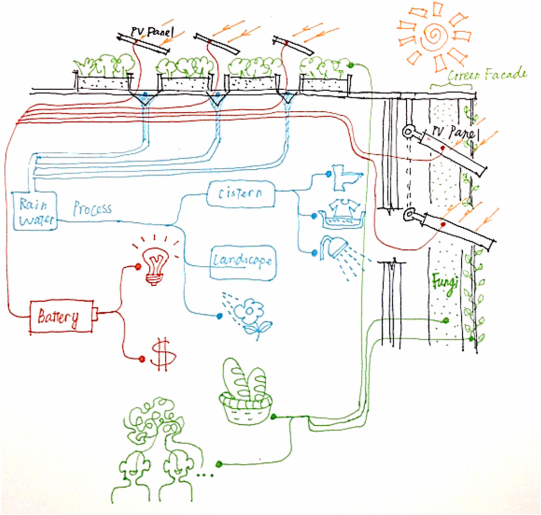
\includegraphics[width=0.8\textwidth]{sketchSustainable.png}
	\caption[System Integration Draft Diagram]{System Integration Draft Diagram}
	\label{fig:sketchSustainable}
\end{figure}
% Chapter 5

\chapter{Drawings} % Main chapter title

\label{Chapter4} % For referencing the chapter elsewhere, use \ref{Chapter1} 

\lhead{Chapter 4. \emph{Drawings}} % This is for the header on each page - perhaps a shortened title

%----------------------------------------------------------------------------------------
\begin{figure}[htbp]
	\centering
		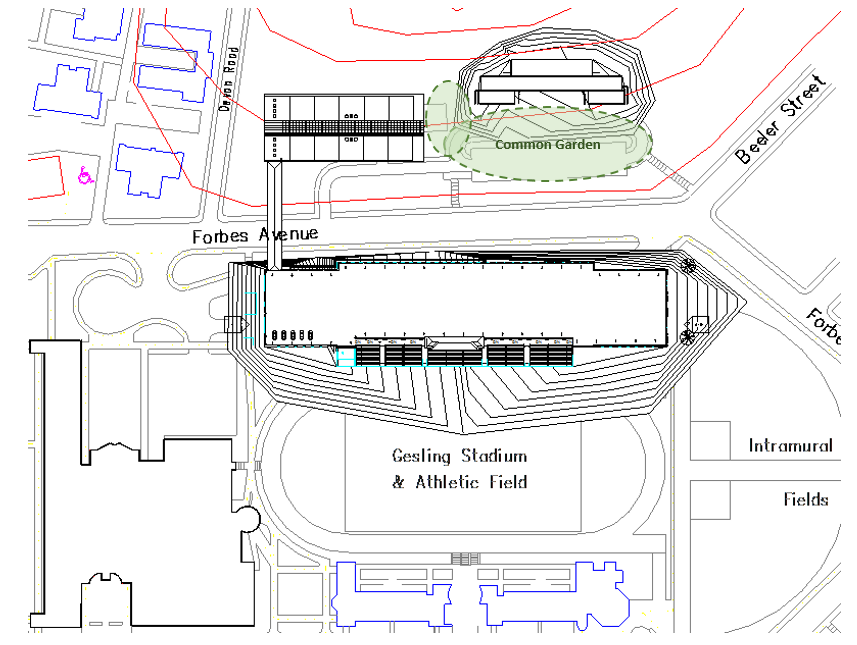
\includegraphics[width=\textwidth]{sitePlan.png}
	\caption[Site Plan]{Site Plan}
	\label{fig:sitePlan}
\end{figure}

\begin{figure}
\centering
\begin{subfigure}{0.5\textwidth}
  \centering
  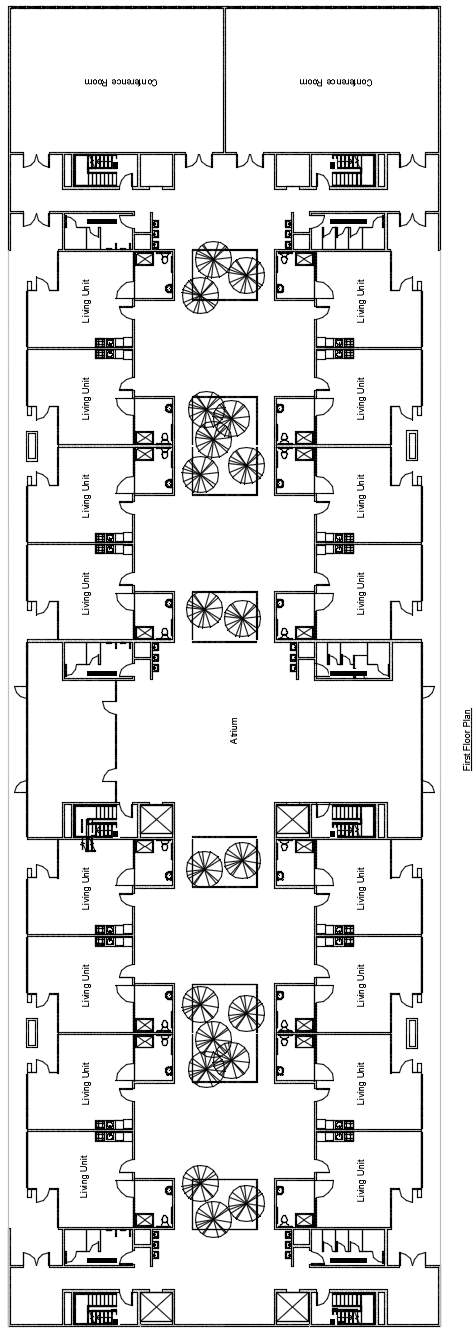
\includegraphics[width=\linewidth]{FirstFloorPlan.png}
  \caption{First Floor Plan}
  \label{fig:FirstFloorPlan}
\end{subfigure}%
~
\begin{subfigure}{0.5\textwidth}
  \centering
  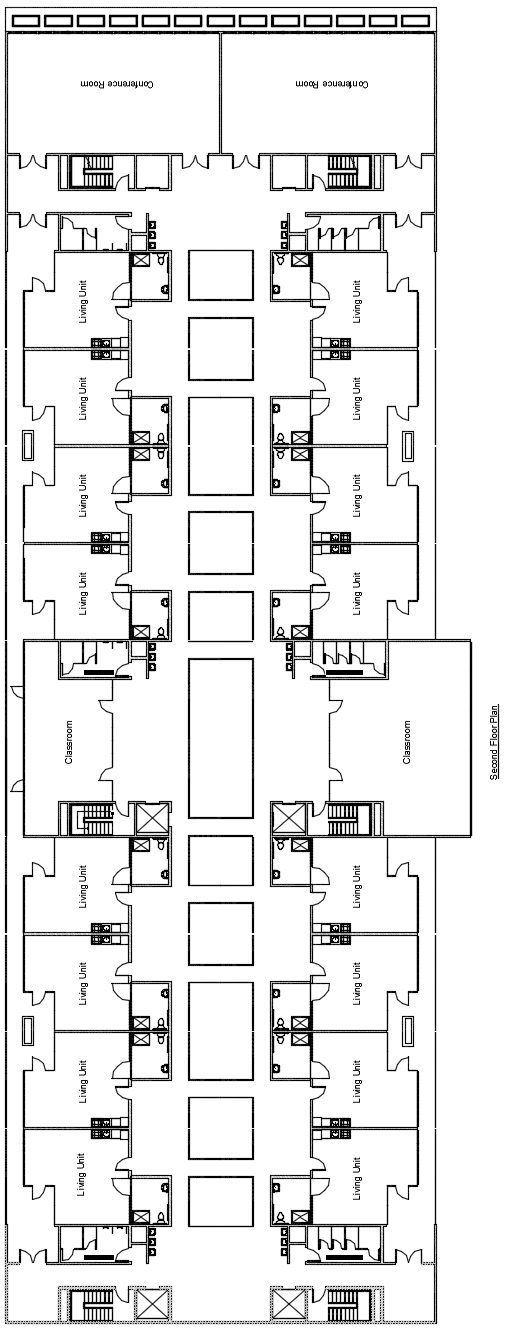
\includegraphics[width=\linewidth]{SecondFloorPlan.png}
  \caption{Second Floor Plan}
  \label{fig:SecondFloorPlan}
\end{subfigure}
\caption{FloorPlan, First Floor and Second Floor}
\label{fig:FloorPlan-Level1-2}
\end{figure}

\begin{figure}
\centering
\begin{subfigure}{0.5\textwidth}
  \centering
  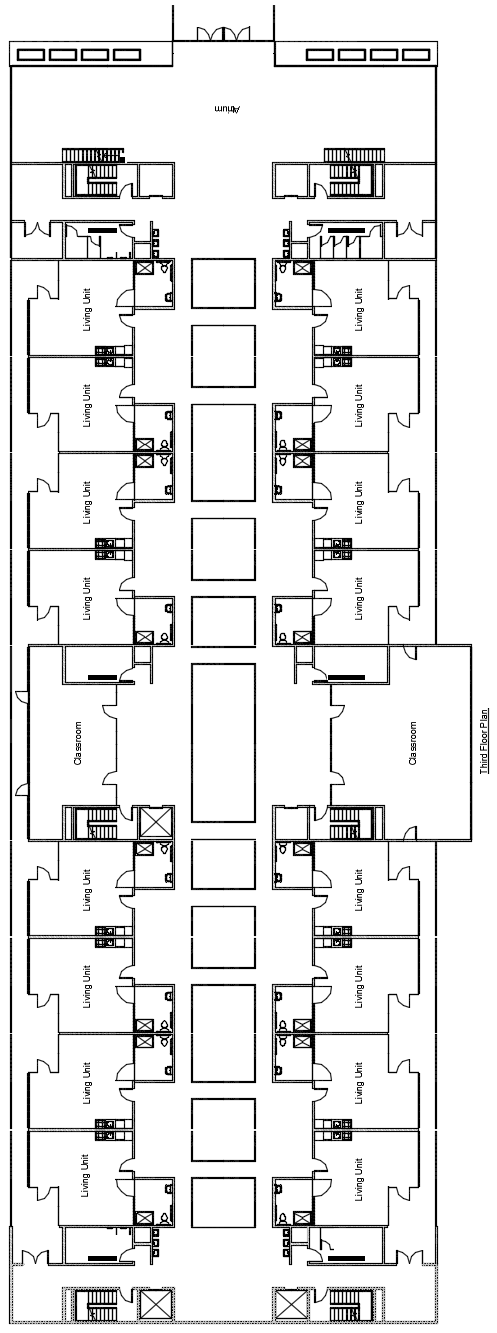
\includegraphics[width=\linewidth]{ThirdFloorPlan.png}
  \caption{Third Floor Plan}
  \label{fig:ThirdFloorPlan}
\end{subfigure}%
~
\begin{subfigure}{0.5\textwidth}
  \centering
  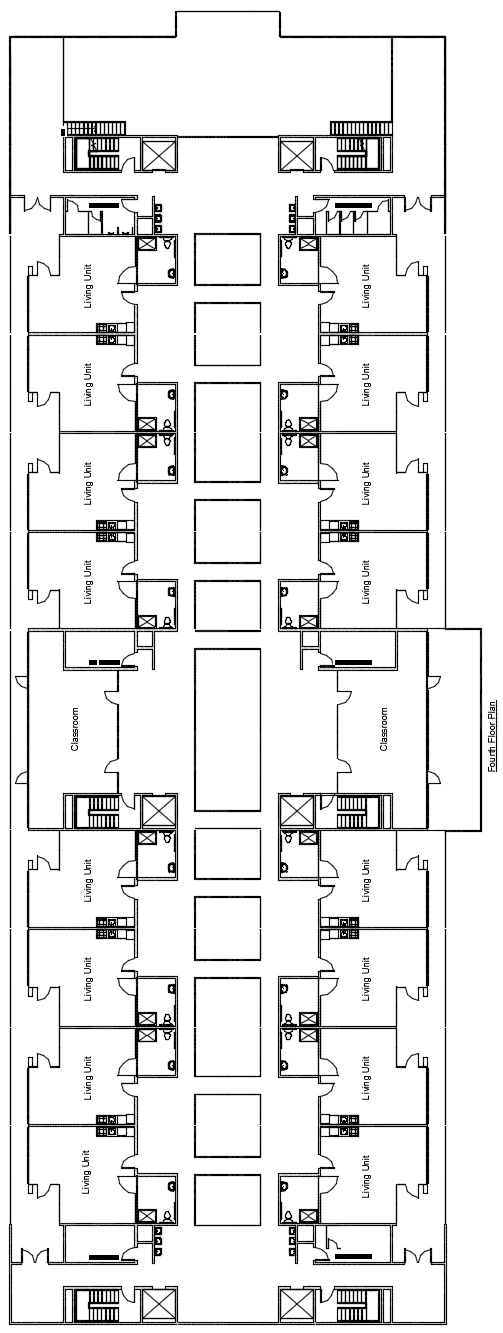
\includegraphics[width=\linewidth]{FourthFloorPlan.png}
  \caption{Fourth Floor Plan}
  \label{fig:FourthFloorPlan}
\end{subfigure}
\caption{FloorPlan, Third Floor and Fourth Floor}
\label{fig:FloorPlan-Level3-4}
\end{figure}

\begin{figure}[t!]
\centering
\begin{subfigure}{0.5\textwidth}
  \centering
  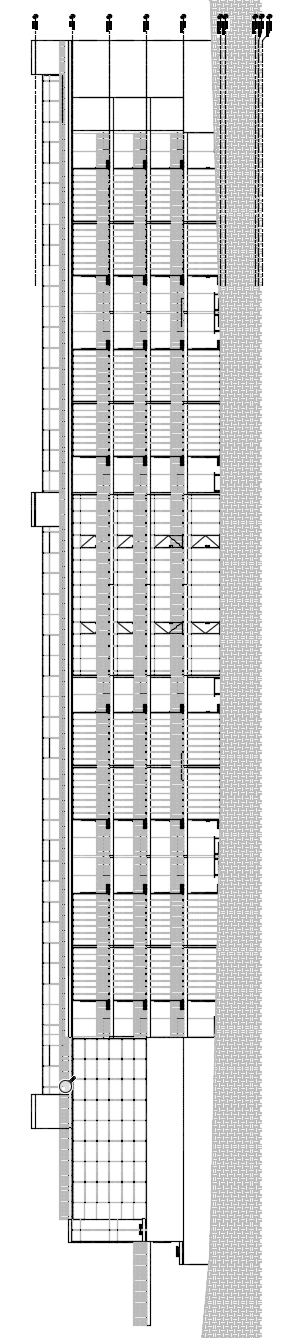
\includegraphics[height = 9in]{ElevationNorth.png}
  \caption{Elevation North}
  \label{fig:ElevationNorth}
\end{subfigure}%
~
\begin{subfigure}{0.5\textwidth}
  \centering
  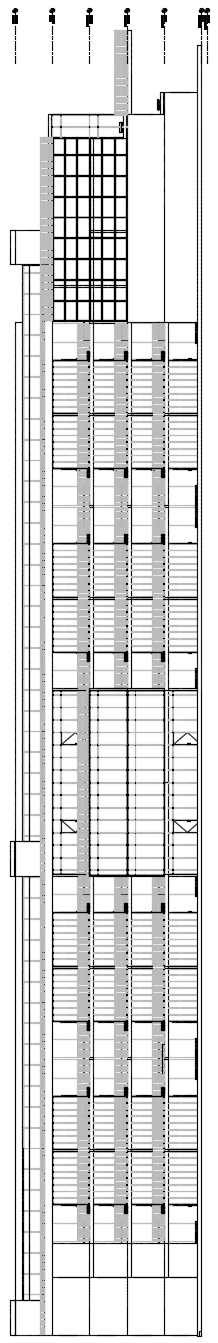
\includegraphics[height = 9in]{ElevationSouth.png}
  \caption{Elevation South}
  \label{fig:ElevationSouth}
\end{subfigure}
\caption{Elevation, North and South}
\label{fig:ElevationNS}
\end{figure}

\begin{figure}[t!]
\centering
\begin{subfigure}{\textwidth}
  \centering
  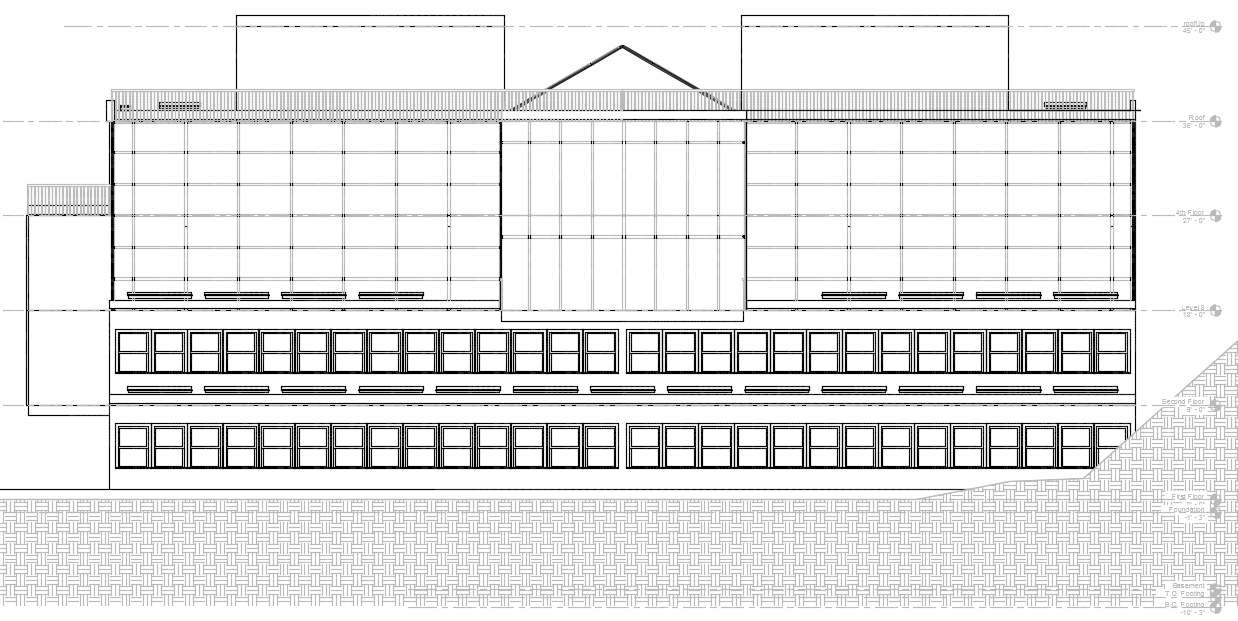
\includegraphics[width = \linewidth]{ElevationEast.png}
  \caption{Elevation East}
  \label{fig:ElevationEast}
\end{subfigure}

\begin{subfigure}{\textwidth}
  \centering
  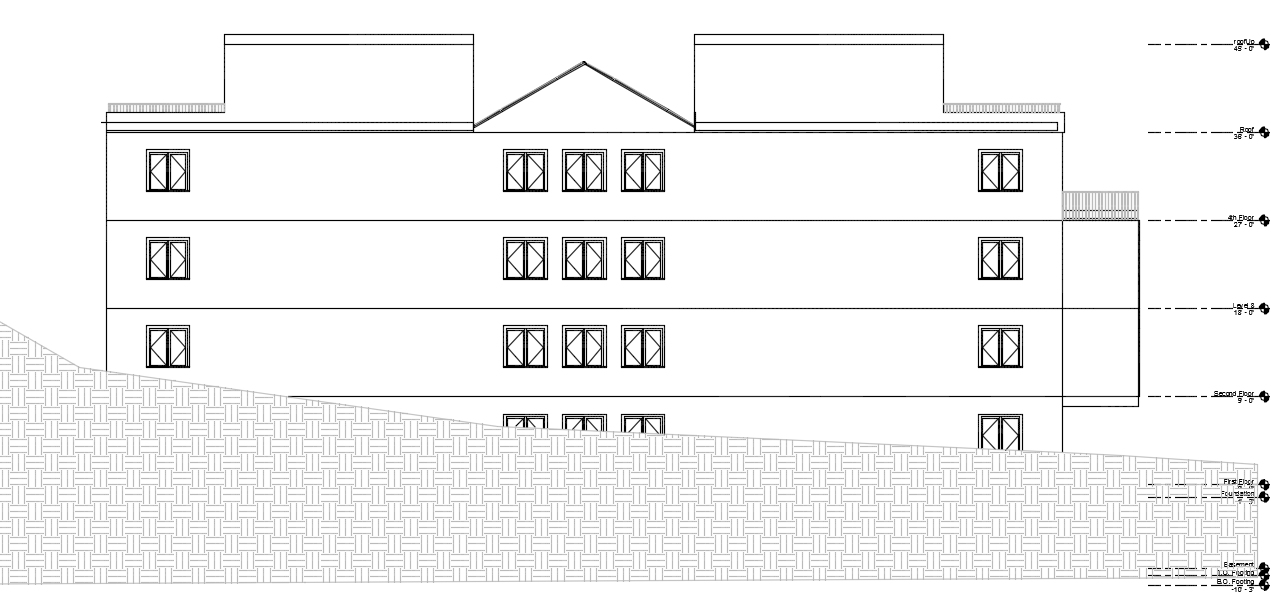
\includegraphics[width = \linewidth]{ElevationWest.png}
  \caption{Elevation West}
  \label{fig:ElevationWest}
\end{subfigure}
\caption{Elevation, East and West}
\label{fig:ElevationEW}
\end{figure}

%\input{Chapters/Chapter5} 
%\input{Chapters/Chapter6} 
%\input{Chapters/Chapter7} 

%----------------------------------------------------------------------------------------
%	THESIS CONTENT - APPENDICES
%----------------------------------------------------------------------------------------

\addtocontents{toc}{\vspace{2em}} % Add a gap in the Contents, for aesthetics

\appendix % Cue to tell LaTeX that the following 'chapters' are Appendices

% Include the appendices of the thesis as separate files from the Appendices folder
% Uncomment the lines as you write the Appendices

%uncomment in final file
% Appendix A
\chapter{List of Existing Senior Center} % Main appendix title

\label{AppendixA} % For referencing this appendix elsewhere, use
                  % \ref{AppendixA}

\lhead{Appendix A. \emph{List of Existing Senior Center}} % This is for the header on each page - perhaps a shortened title
\section{Senior Center Location}
%\begin{tabular}{l{2in}l{2in}r{2in}}
\begin{longtable}{ p{2.5in}| l | l  p{3in}  l}
\toprule
Name&Address&ZIPCODE\\
\midrue
Swissvale Senior Center&7350 McClure Avenue&15218\\
McKinley Park Center&900 Delmont Avenue&15210\\
Leland Resource Center&5230 Wolfe Road&15236\\
Lemington Community Services&1701 Lincoln Avenue&15206\\
Etna Senior Center&18 Walnut Street&15223\\
Millvale Senior Center&917 Evergreen Avenue&15209\\
Allentown - Henry Kaufmann Center&2201 Salisbury Street&15210\\
Allentown - Hilltop Center&631 E. Warrington Avenue&15210\\
Lawrenceville Healthy Active Living Community Center&4600 Butler Street&15201\\
Glen Hazel Healthy Active Living Community Center&945 Roselle Court&15207\\
South Side (Market House) Healthy Active Living Community Center&12th, Bingham Streets&15203\\
Morningside Healthy Active Living Community Center&6944 Presidents Way&15206\\
Homewood Healthy Active Living Community Center&7321 Frankstown Avenue&15208\\
Center Without Walls&901 West Street&15221\\
K. Leroy Irvis Towers&715 Mercer Street&15219\\
Hill House Senior Service Center&2038 Bedford Avenue&15219\\
Hillsdale Resource Center&1444 Hillsdale Avenue Suite 15&15216\\
Knoxville Senior Center&320 Brownsville Road&15210\\
Seton Overbrook Senior Center&2199 Dartmore Street&15210\\
Elizabeth Seton Center&1900 Pioneer Avenue&15226\\
Carrick Senior Center&2019 Brownsville Road&15210\\
Northview Heights Healthy Active Living Community Center&533 Mt. Pleasant Road&15214\\
Northside Healthy Active Living Community Center&5 Allegheny Square&15212\\
Sheraden Healthy Active Living Community Center&720 Sherwood Avenue&15204\\
Brighton Heights Healthy Active Living Community Center&3515 McClure Avenue&15212\\
West End Healthy Active Living Community Center&80 Wabash Street&15220\\
New Image Senior Center&209 13th Street&15215\\
Stephen Foster Center&286 Main Street&15201\\
Forest Hills Senior Center&444 Avenue D&15221\\
PrimeTime Activity Center&440 Lincoln Avenue&15202\\
Plum Senior Center&499 Center - New Texas Road&15239\\
Penn Hills Senior Center &147 Jefferson Road&15235\\
Greenfield Healthy Active Living Community Center&745 Greenfield Avenue&15217\\
Beechview Healthy Active Living Community Center&1555 Broadway Avenue&15216\\
Hazelwoodl Healthy Active Living Community Center&5344 2nd Avenue&15207\\
Mt. Washington Healthy Active Living Community Center&122 Virginia Avenue&15211\\
Jewish Community Center of Greater Pittsburgh&5738 Forbes Avenue&15217\\
"Vintage Inc."&401 N. Highland Avenue&15206\\
Polish Hill Senior Center&30th and Paulowna Streets&15219\\
Braddock Hills Center&3000 Locust Street&15221\\
\caption{Senior Center Location}
\label{tab:seniorCenter}
\end{longtable}
% Appendix A

\chapter{Data Processing Log of GIS Analysis} % Main appendix title

\label{AppendixB} % For referencing this appendix elsewhere, use \ref{AppendixA}

\lhead{Appendix B. \emph{GIS Processing Log}} % This is for the header on each page - perhaps a shortened title
\section{introduction}
The session records the data source and process of using GIS to
conduct the analysis of senior population concentration and existing
senior center.
\section{Process}
\subsection{Building Base Map and Acquiring Geographic Data}
\begin{enumerate}
\item Download Block Group shapefile from Census Bureau
\item Adding the Glock Group layer to the map file
\item Download user tools for retrieving data from the two zip file above~\url{http://www2.census.gov/acs2011_5yr/summaryfile/}
\item Create a gdb folder ``cmu.gdb'' for this assignment and put all related files inside that folder
\item Import the table to the gdb folder
\item Create three new field in attribute table of ``PABlkGrp'':
``senior\_mal''e for male population of above 65 years old,
``senior\_female'' for female population of above 65 years old, one
``totalPopu'' for the total population within a block group.
Join the population table to the layer ``PABlkGrp''
\item Copy and retain the senior population and total population data then remove join
\item Change the projection of the layer of ``PABlkGrp'' from GCS to ``NAD\_1983\_StatePlane\_Pennsylvania\_South\_FIPS\_3702\_Feet'' using Geoprocessing -> Projection and transformation -> Project
\item Calculate senior people percentage over total population with field calculation: [SeniorPopu] / [TotalPopu]
\end{enumerate}
\subsection{Using Geocoding to Add Senior Centers to the Map}
\begin{enumerate}
\item Download table of senior center addresses as a csv file
\item Import the csv file to the cmu.gdb database
\item Use the ``geocoding'' tool in ArcGIS to project the locations of
  senior center to the map as a layer of point features
\item Create a 0.3 mile buffer around the point in the address layer.
\end{enumerate}

%% Appendix A

\chapter{Financial Comparison between Housing Affordability for the Faculty Members} % Main appendix title

\label{AppendixB} % For referencing this appendix elsewhere, use \ref{AppendixA}

\lhead{Appendix B. \emph{Housing Affordability}} % This is for the header on each page - perhaps a shortened title
\section{introduction}
In this section, a rough comparison of the housing affordability for the faculty population between Stanford University and Carnegie Mellon University was conducted. Comparing the median monthly housing cost, we can observe that the median housing cost of Pittsburgh is significantly less than that of Stanford (\tref{tab:midHousingcost}).

\addtocontents{toc}{\vspace{2em}} % Add a gap in the Contents, for aesthetics

\backmatter

%----------------------------------------------------------------------------------------
%	BIBLIOGRAPHY
%----------------------------------------------------------------------------------------

\label{Bibliography}

\lhead{\emph{Bibliography}} % Change the page header to say "Bibliography"

\bibliographystyle{unsrtnat} % Use the "unsrtnat" BibTeX style for formatting the Bibliography

\bibliography{Bibliography} % The references (bibliography) information are stored in the file named "Bibliography.bib"

\end{document}  